\documentclass[twoside,hidelinks]{article}
 
\usepackage[sc]{mathpazo} % Use the Palatino font
\usepackage[T1]{fontenc} % Use 8-bit encoding that has 256 glyphs
\linespread{1.05} % Line spacing - Palatino needs more space between lines
\usepackage{microtype} % Slightly tweak font spacing for aesthetics
\usepackage{geometry} % Document margins
\usepackage{float} % Required for tables and figures in the multi-column environment - they need to be placed in specific locations with the [H] (e.g. \begin{table}[H])
\usepackage{hyperref} % For hyperlinks in the PDF

\usepackage{amsmath}
\usepackage{titlesec} % Allows customization of titles
\titleformat{\section}[block]{\large\scshape\centering}{\thesection.}{1em}{} % Change the look of the section titles
\titleformat{\subsection}[block]{\large}{\thesubsection.}{1em}{} % Change the look of the section titles
\usepackage{algorithm}% http://ctan.org/pkg/algorithm
\usepackage{algpseudocode}% http://ctan.org/pkg/algorithmicx

\algdef{SE}[FOR]{NoDoFor}{EndFor}[1]{\algorithmicfor\ #1}{\algorithmicend\ \algorithmicfor}%


\usepackage{array}
\newcolumntype{C}{>{\centering\arraybackslash}p{13ex}}
\usepackage{multirow}
\usepackage{fancyhdr} % Headers and footers
\pagestyle{fancy} % All pages have headers and footers
\fancyhead{} % Blank out the default header
\fancyfoot{} % Blank out the default footer
\fancyhead[C]{Master thesis $\bullet$ Panagiotis Chatzichristodoulou $\bullet$ 2015} % Custom header text
\fancyfoot[RO,LE]{\thepage} % Custom footer text

 
\usepackage{wrapfig}
\usepackage{graphicx}
\graphicspath{ {pics/} }
\usepackage{paralist}
%----------------------------------------------------------------------------------------
%	TITLE SECTION
%----------------------------------------------------------------------------------------

\title{
\Huge{Master Thesis} \\
\noindent\rule{4cm}{0.4pt} \\
\vspace{5mm}
\huge{\selectfont{Towards lifelong mapping in pointclouds}}
\vspace{5mm} \\
\normalsize Panagiotis Chatzichristodoulou \\
\noindent\rule{4cm}{0.4pt} \\
\vspace{5mm}
\fontsize{24pt}{10pt}{Master Thesis DKE 09-16 }} % Article title

\author{
\normalsize Thesis submitted in partial fulfillment\\
\normalsize  of the requirements for the degree of Master of Science \\
\normalsize of Artificial Intelligence at the Department of Knowledge \\
\normalsize  Engineering of the Maastricht University \\
\vspace{5mm} \\
\normalsize \textbf{Thesis Commitee:} \\ 
\normalsize University of Maastricht \\ % Your institution
\normalsize \textit{Rico Mockel, Kurt Driessens} \\
\normalsize Distributed Organisms B.V.(DoBots)\\
\normalsize \textit{Anne Van Rossum} \\
\vspace{0mm} \\
\normalsize Maastricht University \\
\normalsize Faculty of Humanities and Sciences \\ 
\normalsize Department of Knowledge Engineering \\
\normalsize Master Articial Intelligence \\
}


%----------------------------------------------------------------------------------------

\begin{document}

\maketitle % Insert title

\thispagestyle{fancy} % All pages have headers and footers

%----------------------------------------------------------------------------------------
%	ABSTRACT
%----------------------------------------------------------------------------------------
\newpage
\begin{abstract}

\noindent Long term mapping is the natural conceptual extension to existing mapping methods that are focused on mapping static environments.
Existing methods do not address problems such as memory restrictions and changes that occur in map over time. Therefore, if tackled efficiently, the solution of lifelong mapping will be one important step towards fully autonomous robots.
As discussed in the literature, lifelong mapping consists of two major subproblems. A compression problem as the size of the map increases over time, and a dynamic environment problem as the environment changes over time. This thesis investigates the application of non-parametric Bayesian methods and how such tools can be used to tackle the compression subproblem of lifelong mapping methods. A novel method of pointcloud representation is introduced and its results are applied to an extended Kalman filter algorithm; both its compression strength and expressive power are analyzed, as are directions in which the method could be improved and extended to formulate a general solution to both the compression as well as the dynamic environment problem of lifelong mapping.


\end{abstract}

%----------------------------------------------------------------------------------------
%	ARTICLE CONTENTS
%----------------------------------------------------------------------------------------
 
\tableofcontents
\listoffigures
 
 

\newpage


\section{Introduction}
\label{sec:Intro}

\subsection{Motivation}


Simultaneous Localization And Mapping(SLAM) is one of the fundamental challenges of autonomous systems\cite{probRobs}. 
In order for robots to be considered truly autonomous they have to be able to navigate through an unknown environment whilst mapping its structure.
With solutions like EKF-SLAM\cite{ekf} and FastSlam\cite{SLAM} robots are currently capable of efficiently mapping unknown environments. 
Methods that remove the restrictions of mapping \textit{static} environments for a \textit{finite} amount of time are the logical extension to existing methods.
Lifelong learning in robots is not a new concept\cite{liflonglearning}; in recent years research with a specific focus on lifelong learning in mapping\cite{lifelongmaps} was introduced.  Lifelong mapping introduces the concept of robots that are capable of continuously mapping their environment with this leading to two basic extensions over existing methods: Mapping methods that are capable of handling the memory needs of a constantly increasing environment and robust enough to handle changes that occur in the environment over time. 

The increasing need of memory resources brings in the spotlight one of the fundamental restrictions of autonomous systems, i.e. memory bottlenecks. In order to be able to map an unknown environment for an arbitrary amount of time, an arbitrary amount of memory is required. Since memory resources can only be finite, the need for methods that store environment information in a less costly manner rises. The problem then transposes to a compression problem with two basic questions: How can environment information be compressed? How do we minimize information loss due to the compression?

As a result, lifelong mapping consists of two basic subproblems: a compression problem as the map increases over time and a dynamic environment problem as the environment changes over time\cite{aishalong}. In this thesis the focus will be directed on the compression problem of lifelong mapping. More specifically, how can Bayesian non-parametric methods be used to create compressed environment representations that still retain enough environment information after the compression takes place. Since different sensors require different mapping approaches the focus will be directed towards algorithms that use RGBD sensors like Microsoft Kinect to perform the mapping. 

\subsection{Tools and methods}
Dirichlet processes and Dirichlet process mixture models \cite{nonParam} are the cornerstone of Bayesian non-parametric statistics. The strength of those models lies in the fact that they allow their components to grow as much as needed so as to best fit the data; this means that in such models you must not predefine the number of topics in a corpus of documents, the number of objects in a picture or items in a point cloud. This implied information that resides in the data can be infered by the models themselves. The dynamic number of components in combination with different prior choices leads to very flexible solutions that can be used in a very large area of applications from topic modeling\cite{LDA} to speaker diarization\cite{speakerDiar}.
The main motivation of this thesis is to use such methods as a means of creating compressed representations of the environment that also carry a high amount of information the initial data did. 

Since its introduction in 2010 Microsoft Kinect\cite{kinect} has revolutionized RGBD devices with its low price range and high quality sensors. It came as no surprise that research in pointclouds, the cloud representation system of Kinect, has increased since then. Many libraries that enable the user to perform tasks from feature extraction to plane segmentation\cite{pcl} in pointclouds are currently available. In the field of robotics, many teams are using the Kinect sensors to perform simultaneous localization and mapping\cite{rtabmap},\cite{rgbdmapping}. The goal of this thesis is to introduce a compressed representation of pointclouds in order to tackle the first part of lifelong mapping problems while using Bayesian methodologies. 


\subsection{Research questions}


The following research questions have then to be addressed: Are such representations rich enough to be used as sensor models in SLAM?  Will the methods be fast enough to be used in online SLAM scenarios? Will the compression ratio with respect to normal repesentations be significant? 

In this thesis a method of creating compressed representation of a pointcloud is introduced; the representation's compression strength, expressive ability as well as the ability to handle online streams of data are presented in the results section. The discussion section analyzes some details regarding the mechanisms of the method, cases where the method does not perform as expected, as well as implications of having a method that has an unsupervised learning engine at its core.

The rest of the paper is structured as follows. Section \ref{sec:literature} will present relevant literature review, section \ref{sec:theory} will introduce the theories behind the model, section \ref{sec:model} will define the model, section \ref{sec:results} will show experimental results of the method. Section \ref{sec:discussion} will discuss specific behaviours of the method and, finally, section \ref{sec:conclusion} will conclude with a short summary and future extensions by which the method could be improved.

%------------------------------------------------

\newpage
\section{Literature review}
\label{sec:literature}

Literature review will be focused on 4 related sub fields: Object based SLAM, methodologies pointcloud object segmentation, non-parametric Bayesian methods and the correspondence problem in SLAM.

Given that the basic motivation of the thesis is to create representations of objects within the cloud, methods that use objects to perform SLAM are relevant. The second part of the literature research is focused on pointcloud segmentation and the features that need to be extracted from a cloud to minimize information loss. The third part of the research is focused on non-parametric Bayesian methods and the clustering tools they provide. Finally, literature review is focused on the correspondence problem in SLAM. As one of the fundamental problems that need to be solved in order to have robust SLAM algorithms, it is imperative the correspondence problem be solved efficiently. 

\subsection{Object based SLAM}


Object based SLAM introduces a specific category of mapping problems where objects are used as reference points while navigating through the environment.
Salas-Moreno et al.\cite{SLAM++} define a method of performing object based SLAM for specific classes of objects. The objects are identified by a camera that is on top of the robot. By having a model of pre-trained objects, SLAM can be performed on environments where the robot knows what objects to expect.
Castle et al. use object recognition to perform object based SLAM with the use of a hand-held cameras. Selvatici et al.\cite{objSLAM} use a similar approach while exploiting structural information such as object height and position within the room. That way a couch that is a large object situated in floor level is easier to be recognized.
Choudhary et al.\cite{objectpointSLAM} use pointclouds and an object database to match objects currently seen with known objects within their database. They use omnimaper\cite{omnimaper} as their mapping method, and as their representation a combination of the downsampled voxel grids with additional normal and curvature information.  Finally, all their operations are done in the non-planar components of the pointcloud.
Jensfelt et al\cite{objSLAM} present an object based approach to SLAM where the robot can manipulate the objects of the map. They use camera pictures as input and receptive Field Histogram as the method to abstract the camera input and extract features for their object matching algorithm. Their approach is proposed as a solution to a service robot scenario.
MonoSLAM\cite{monoSLAM} introduces a method of performing SLAM using a monocular camera. 
Seongyong Koo et al.\cite{objectDisc} introduce a method of unsupervised object individuation from RGB-D image sequences. They cluster their initial cloud into candidate objects using Eucledian clustering and proceed to extract features like the Euclidian distance(L2) and the Kullback-Leibler divergence between pointcloud objects. They use IMFT to solve their tracking problem.

The common base of such methods, with the exception of \cite{objectDisc}, is that they treat the problem of object based SLAM as a classification task. More specifically, the robot can navigate in environments where it knows what objects to expect.
The approach presented in this paper introduces a general and unsupervised method of using environment signatures as reference points to perform SLAM.

\subsection{Point Cloud Object clustering}


Point cloud clustering tools enable the user to cluster clouds in objects, or segments of structure that "make sense". The robustness of the clustering varies with respect to the method used the features it requires as well as the application domain.
Trevor et al.\cite{pointSeg} take positional information, Euclidean distances and the normal of points to as input to their function and output segments that are part of the same object. PCL library\cite{pcl} introduces methods like Euclidean clustering and conditional Euclidean clustering that use a number of heuristics that take normal as well as curvature information to extract segments in the pointcloud that represent objects. Furthermore, there is a lot of research on segmentation of pointclouds in scenes, with the emphasis usually put on extracting geometric primitives\cite{planarSeg},\cite{planarSeg2} using cues like normals and curvature. Rabbani et al.\cite{segOverview} introduce a new method of object segmentation using KNN as their base algorithm. They also present a very informative literature review along with the strengths and weaknesses of existing methods. Finally Triebel et al.\cite{smartSeg} introduce a general clustering framework that does not rely on plane segmentation. Instead of segmenting the plane by using classical approaches like RANSAC or MLASAC they introduce a framework where they make no assumptions regarding plane data. 
 
In this thesis an alternative novel clustering approach will be introduced that will use Bayesian non-parametric methods as its base.

\subsection{Non Parametric Bayesian methods}

Dirichlet processes and Dirichlet process mixture models are the cornerstone of Bayesian statistics. In this thesis the focus is directed towards the clustering methods that are being introduced by those tools. Radford M. Neal\cite{bayes:neal} with his paper regarding Markov Chain Monte Carlo(MCMC) methods for Dirichlet process mixture models made the definitive step towards Dirichlet Process Mixture Models(DPMM's) receiving a lot of attention. Since then, a variety of approaches for inference on such models has been introduced with MCMC methods, and Variational Inference(VI) methods being two prominent such approaches. Variational inference for Dirichlet Process Mixture Models(DPMM), introduced by Jordan et al.\cite{bayes:jordan} introduces deterministic tools to perform inference and approximate the posterior distribution and marginals of a dataset. Blei et al.\cite{LDA} introduced Latend Dirichlet Allocation(LDA) as a method to perform topic modelling. Teh et al.\cite{bayes:hier} add a level hierarchy on the inference process by introducing the Hierarchical Dirichlet process. Particle filter approaches have also been established. Doucet et al.\cite{bayes:smc} introduce Sequential Monte Carlo(SMC) as a fast way to approximate inference. Dirichlet process mixture models are a very active research field and covering it is beyond the scope of this thesis. 

In this thesis SMC samplers where used due to their robustness as well as their inherent extensiveness. A detailed description on the mechanisms of sequential samplers will be given in the theory section.

\subsection{Correspondence}

In its general definition, the correspondence problem refers to the problem of ascertaining which parts of one image correspond to which parts of another image, where differences are due to movement of the camera, the elapse of time, and/or movement of objects in the photos. Under the object based SLAM context, correspondence refers to the problem of identifying objects as ones that have been encountered before during the mapping process. In that direction, Cree et al.\cite{corresp:first} create a histogram of line segments of each landmark and compute their root mean square error. They then proceed to calculate their RGB signature to calculate the distance between different landmarks. Low et al.\cite{corres:sec} match Scale Invariant Feature Transform (SIFT) features, an approach which transforms image data into scale-invariant coordinates relative to local features. Lamon et al.\cite{corres:three} store a database of fingerprints which indicate the location in the robot's environment. The features are ordered and stored at a database as they appear in the robot's immediate surroundings. A new fingerprint is computed for each new view and matched against existing ones. Finally, in Seghal et al.\cite{corres:four} an extension of SIFT descriptors to 3D data and pointclouds is given. 

In this thesis the correspondence problem is solved using a simple decision layer that compares current environment signatures to past ones.

%------------------------------------------------

\newpage
\section{Theory background}
\label{sec:theory}


An introduction to the Dirichlet Distribution and Dirichlet process mixture models will be given. Finally, the Generaly Polya urn model will be presented as it serves as the base to the sampler presented in the model section.

\subsection{Dirichlet Distribution}

An example of a \textit{probability mass function}(pmf) can be described through an ordinary six-sided dice. To sample from this function, you cast the dice and get a number from 1 to 6. One important property of probability mass functions taken from real dice is that they are not uniformly weighted due to the manufacturing process not being perfect. A bag of dice can then be considered as an example of a random pmf. To sample from this random pmf, you have to put your hand in the bag and draw a dice, and the result of this drawing process is itself a probability distribution. A Dirichlet distribution is an object that can be used to model the randomness of such objects whose domain is itself is a probability distribution i.e it is a distribution of distributions.

Formally, a probability density function with \textit{k} components lies on the \textit{(k-1)} dimensional probability simplex, which is a surface in $ \mathbb{R}^k $ denoted by $ \Delta_k $ and defined to be the set of vectors whose $ k $  components are non-negative and sum up to 1, that is:  $ \Delta_k = \{ q \in  \mathbb{R}^k | \sum_{i=1}^k q_i=1, q_i \geq 0\ for\ i=1,2,...k \} $ . $ \Delta_k $  is itself a $ ( k-1 ) $ dimensional object lying in the $k$ dimensional space. 

\textbf{Dirichlet distribution:} Let $ Q = [Q_1,Q_2,...,Q_k  ] $ be a random pmf, that is, $ Q_i \geq 0 $ for $ i=1,2,..k $ and $ \sum_{i=1}^k Q_k=1 $. In addition, suppose that $ \alpha = [\alpha_1, \alpha_2, ..., \alpha_k ] $, with $ \alpha_i  \ge  0 $ for each i, and $ \alpha_0 = \sum_{i=1}^k \alpha_i $. Then $ Q $ is said to have a Dirichlet distribution with parameter $\alpha$, which we denote by $ Q \sim  Dir(\alpha)$, if it has $f(q;a) = 0$ if q is not a pmf, and if q is a pmf then f has a probability density function of:
\begin{equation}
 f(q; \alpha) = \frac{ \Gamma( \alpha_0)  }{ \prod_{i=1}^{k} \Gamma ( \alpha_i) } \prod_{i=1}^{k} q_i^{a_i -1}
\end{equation}
The first two cumulants of the distribution are the following:

\begin{equation}
 E[ \alpha_i]\ =\ \frac{ \alpha_i }{ \alpha_0 } 
\end{equation}

\begin{equation}
 Cov(Q_i,Q_i) =
\left\{
	\begin{array}{ll}
		\frac{ - \alpha_i \alpha_j }{ \alpha_0^2 ( \alpha_0+1) }                   & \mbox{if } i \neq j  \\
		\frac{ - \alpha_i ( \alpha_0 - \alpha_i) }{ \alpha_0^2 ( \alpha_0+1)} & \mbox{if } i=j
	\end{array}
\right.
\end{equation}
Mean and variance formulas help understand how the changing the $ \alpha $ vector affects the behaviour of the distribution as to where the density is located as well as the variance in the pmfs sampled. The following graphs display the difference of behaviour on samples from Dirichlet distributions with different initial $\alpha$ values.


Random samples from a Dirichlet distribution are presented in Fig.\ref{firstplot}. It must be noted that every point within the simplex can be considered itself a pmf since its components add up to one.  Furthermore, for an $ \alpha = [c,c,c]\ ,c \ge 0 $ , the density is symetric towards the center of the simplex; the special case of $ \alpha = [1,1,1] $ with c=1 is displayed at Fig.\ref{firstplot}(a) where the initial choice of the $\alpha$ vector results is a uniform distribution of points over the probability simplex. As c increases the distribuiton is concentrated towards the center of the simplex. The behaviour of the density changes when the $\alpha$ vector is not symetric, when there is a shift in density towards the higher parameter, as is shown in Fig.\ref{firstplot}(b) and Fig.\ref{firstplot}(c). Finally, when the values of the vector are smaller than 1, the density of the distribution is shifted towards the vertices of the simplex as is shown in subplot Fig.\ref{firstplot}(d).
    \begin{figure}[!h]
        \begin{tabular}{cc}
       	          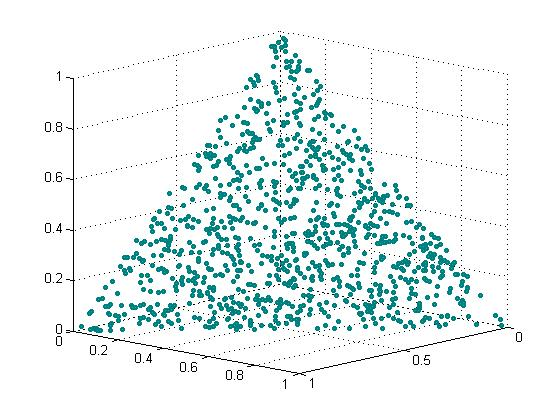
\includegraphics[width=0.35\textwidth]{uniformDist} & 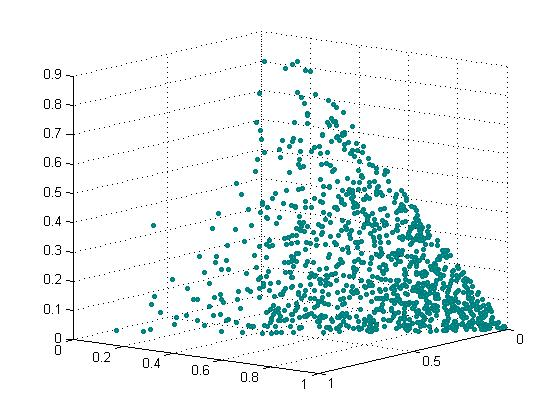
\includegraphics[width=0.35\textwidth]{1-3-1Ddist} \\
    		(a) $ \alpha = [1,1,1] $ & (b) $ \alpha = [1,3,1] $  \\[6pt]
    		 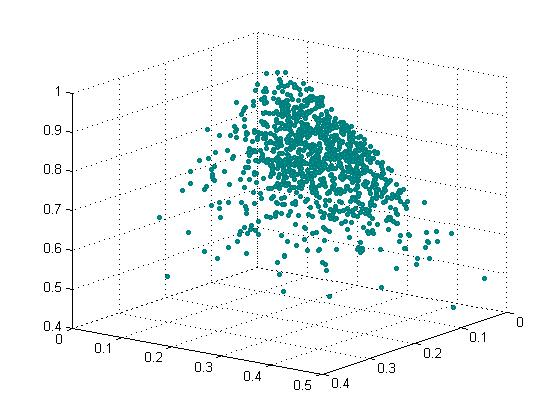
\includegraphics[width=0.35\textwidth]{2-5-20Dist} &    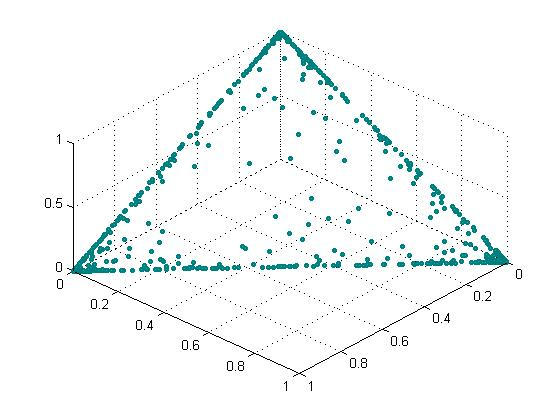
\includegraphics[width=0.35\textwidth]{01-01-01Dist} \\
    		(c) $ \alpha = [2,5,20] $  & (d) $ \alpha = [0.1,0.1,0.1] $  \\[6pt]
    	\end{tabular}
    	\caption{Different behaviour the distribution for different initial parameters of the $\alpha$ vector}
    	\label{firstplot}
     \end{figure}

One important property of the Dirichlet distribution is that it serves as a conjugate prior to the probability parameter $q$ of the multinomial distribution. 

That is,  if $ X|q \sim\ Multinomial_k(n,q) $ and $ Q \sim Dir( \alpha ) $ then $ Q| X=x \sim Dir( \alpha + x) $

\subsection{Sampling methods}

Two basic sampling methods from the Dirichlet Distribution will be presented: Stick breaking process, and Polya's urn.

\subsubsection{Stick breaking process}

The stick breaking process can be though of as follows: Imagine breaking a unit length stick into $k$ such that the $k$ pieces follow a $Dir( \alpha)$  distribution. Such samples can be created by the following procedure:
\begin{compactitem}
	\item  \textbf{Step 1:} Simulate $ u_1 \sim Beta(a_1, \sum_{i=1}^k a_i ) $, and set $q_1 = u_1$. That's the first piece of the stick, with the remaining piece having length of $ 1-u_1$
	\item \textbf{Step 2:} For $ 2 \leq j \leq k-1$, if j-1 pieces, with lengths  $u_1,u_2,...,u_{j-1},..$ have been broken off, the length of the remaining stick is $\prod_{i-1}^{j-1} (1 - u_i) $. We simulate $ u_j \sim Beta( a_j, \sum_{i=j+1}^k a_i) $ and set  $q_j=u_j \prod_{i=1}^{j-1}(1-u_i)$. The length of the remaining part of the stick is  $\prod_{i=1}^{j}(1-u_i)$
	\item  \textbf{Step 3:} The length of the remaining piece is $q_k$.


\end{compactitem}
Since the last part of the stick will always be created so that we end up with a valid pmf, it is made explicit how the density of the Dirichlet is  a ${k-1}$ dimensional object lying in the $k$ dimensional space. Fig.\ref{stickR3} shows realizations of of the stick breaking process in $R^3$ and the similarities between the stick breaking sampling method and the probability simplex presented in the previous section are shown.

\begin{figure}[!h]
    \centerline{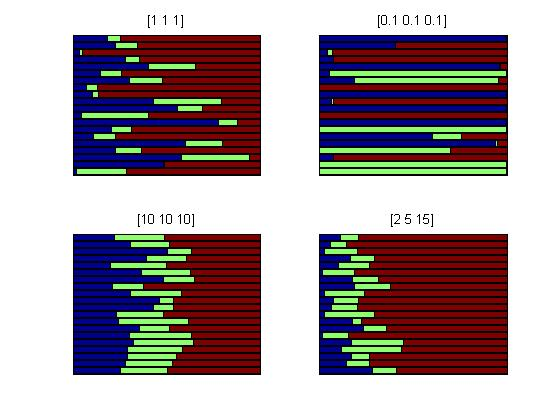
\includegraphics[width=.55\textwidth]{stickBreaking}}
    \caption{Realizations from a Dirichlet distribution using the stick breaking construction in $R^3$. Each color represents the weight of the respective component. Weights sum up to 1 making every realization a probability mass function. A single line can be mapped to a single dot in Fig. \ref{firstplot}  }
\label{stickR3}
\end{figure}


As expected, an initial $\alpha$ vector of [1,1,1] results in a uniform distribution of weights. Furthermore, as the weights in the $\alpha$ vector increase we have a more balanced distribution of weights as shown for the case of Fig.\ref{stickR3}([10,10,10]) and this this balance is shifted towards the higher weight when the initial vector is not symmetric as shown in Fig.\ref{stickR3}([2,5,15]). Finally, an initial vector of weights $<1$ results in single values dominating the simplex.
\subsubsection{Polya's Urn}

The second method of sampling from a Dirichlet distribution is by using an urn model. In probability theory and statistics, an urn problem is an idealized mental exercise in which some objects of real interest are represented as colored balls in an urn or other container. More specifically, Polya's urn model depicts a random process whose realizations are realizations of a Dirichlet distribution.
\begin{figure}[!h]
    \centerline{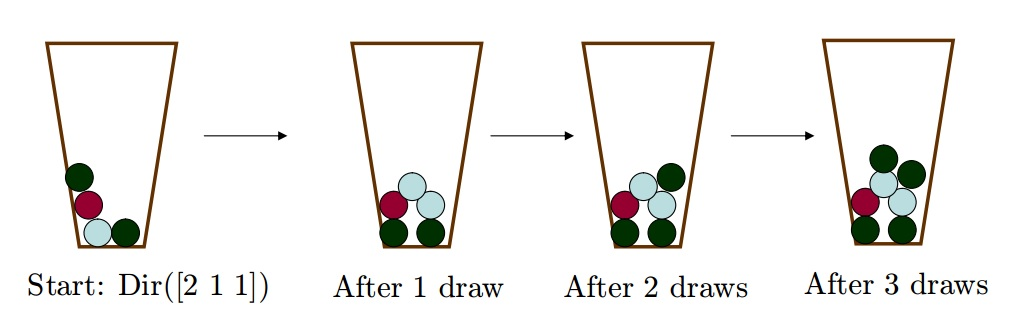
\includegraphics[width=0.5\textwidth]{urn}}
	\caption{Polya's urn for $\alpha$=[2 1 1] }
	\label{polysurn}
\end{figure}
Supose that you want to generate $Q \sim Dir( \alpha ) $.To start, we put $\alpha_i$ balls of colour i for $i=1,2,...,k$ in an urn, as shown in Fig.\ref{polysurn}. It must be noted that $\alpha$ can be fractional and even irrational(!). At each iteration we randomly draw a ball from the urn and put it back in the urn with an extra ball of the same colour as well. As we iterate this procedure an infinite amount of times, the proportions of the balls of each colour will converge to a pmf that is a realization of from the distribution $Dir(\alpha)$.

The procedure can be then described as follows:
\begin{compactitem}

	\item \textbf{Step 1:} Set a counter n=1. Draw $ X \sim \alpha / \alpha_0 $. 
	\item \textbf{Step 2:} Update counter to n+1. Draw $ X_{n+1} | X_1, X_2, ..., X_n \sim \alpha / \alpha_{n0}$, where $\alpha_n = \alpha + \sum_{i=1}^n \delta_{X_i} $ and $ \alpha_{n0}$ is the sum of the entries of $\alpha_n$. Repeat step 2 an infinite number of times.
\end{compactitem}

As the number of iterations of Step 2 approaches infinity, the proportions of ball colors in the simplex will be a realization from the distribution $Dir(\alpha)$with an initial vector $\alpha$.



\subsection{Dirichlet Process}

The Dirichlet process was formally introduced by Thomas Ferguson in 1973 and serves as an extension to the Dirichlet distribution in modelling infinite sets of events. More specifically, in the introductory example, a six sided dice was described. If instead of a six sided dice a dice with an infinite amount of sides was used, the Dirichlet Distribution could not handle the infinity of the sample space. A Dirichlet process is a random process whose realizations are distributions over an arbitrary and possibly infinite sample space. To make the infinity assumption manageable, the Dirichlet process restricts the class of distributions it can handle to a specific set: Discrete distributions over the infinite sample space that can be written as an infinite sum of indicator functions which can be formally presented as:

\begin{equation}
 P( B ) = \sum_{k=1}^\infty p_k \delta_{y_k} 
 \end{equation}

Where $p_k$ is the mixture weight and $\delta_{y_\kappa}$ is an indicator function such that $\delta_{y_\kappa} (B)=1\ if\ y_{\kappa}\ \in B$ and  $\delta_{y_\kappa}(B)=0$ otherwise. This formulation makes explicit the fact that realizations of a Dirichlet process are discrete distributions.

Formaly, the DP is defined as follows: Let $\mathcal{X}$ be a set and let $\mathcal{B}$ be an $\sigma$-algebra on $\mathcal{X}$ .  Let ($\mathcal{X} $, $\mathcal{B}$ )  denote the collection of probability distributions on set as $\mathcal{P} $. $\mathcal{P}$ is a Dirichlet Process as with a strength parameter $\alpha$ and a base distribution $H$ on ($\mathcal{X} $, $\mathcal{B} $ ) if for any finite measurable partition $ \{B_i\}_{i=1}^k$ of $\mathcal{X} $, the random vector (($ P(B_1), ..., P(B_k)$) has a Dirichlet distribution with parameters (($ \alpha H(B_1), ..., \alpha H(B_k)$) . The mean and the covariance of a Dirichlet process are defined as:
\begin{itemize}

	\item{ $ \mathcal{E}[G(A)] = \alpha H(A) $. The base distribution can be though of as the mean of the Dirichlet process}

	\item{$ \mathcal{V}[G(A)] = \frac{H(A)(1-H(A))}{\alpha + 1} $. The strength parameter $\alpha$ can be though of as the inverse covariance of the Dirichlet process. }
\end{itemize}

\subsection{Sampling methods}

Two methods for sampling from a Dirichlet process will be presented: the Chinese Restaurant Process, the Stick breaking process.


\subsubsection{Chinese restaurant process}
\label{sec:crp}
Polya's Urn and the stick breaking process are two names of the same process. The chinese restaurant process paradigm is similar to the Polya's urn and it is defined as follows:
Imagine a restaurant with an infinite number of tables, each with infinite capacity. At time t=1, the first customer enters the restaurant and sits at table 1 with probability 1. For every next step, the customer can either

\begin{compactitem}
	\item Choose an unoccupied table with probability $ \propto \frac{\alpha}{n-1+ \alpha }$
	\item Choose occupied table k with probability $ \propto  \frac{c}{n-1+ \alpha }$ where c is the number of people currently sitting at that table
\end{compactitem}


If you let an infinite number of customers enter the restaurant, the proportions of people sitting on each table will be a realization from a Dirichlet process with strength parameter $\alpha$.

It can be seen that there is a positive reinforcement effect in this process, that is the more people already sitting at a table, the bigger the probability that more people will be sitting into that table in the future. It can also be proved that the number of tables grows $ \propto \alpha log(n)$ where n is the number of customers in the restaurant. Fig.\ref{CRP} visualizes the progression of the proccess as more people enter the restaurant. 

\begin{figure}[!h]
          \centerline{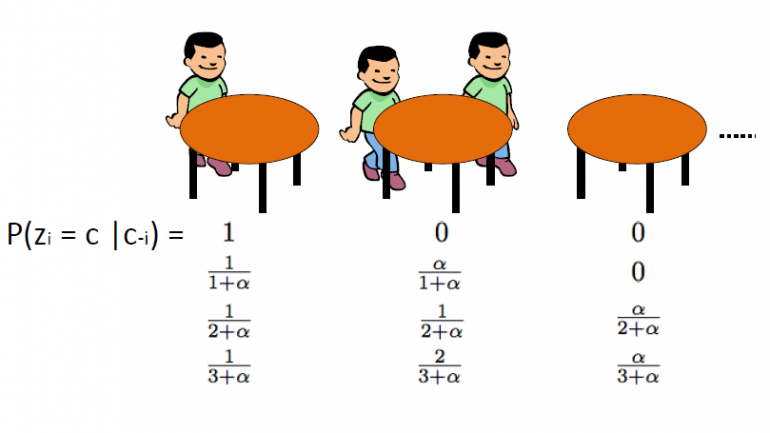
\includegraphics[width=.70\textwidth]{crp}}
	\caption{The CRP process}
	\label{CRP}
\end{figure}


One important property of this procedure is that the nth customer has the same probability to sit on the same table as any other customer of the table. That is the number of people seating on table 1 is on average the same as the number of people seating on table $k$! This very interesting and counter intuitive(at first) property of the exchangeable data and understanding this is crucial on building intuition regarding the behaviour of exchangeable random variables.


\subsubsection{Stick breaking}

Measures drawn from a Dirichlet distribution are discrete with probability 1. This property is made explicit by the stick breaking process. The construction is based on the independent sequences of i.i.d. random variables $(\pi'_k)_{k=1}^\infty$ and $ ( \phi_k)_{k=1}^\infty$  defined as follows:


  \begin{equation}
\pi'_k  | \alpha_0, G_0 \sim Beta(1, \alpha_0)\ \ \ \ \ \ \ \ \ \   \phi_k | \alpha_0, G_0 \sim G_0
\end{equation}



This can be defined as follows: Draw $\pi'_k$ as a Beta random variable. Draw $\phi_k$ from $G_0$ Now define a random measure G as:


\ \
\begin{equation}
\pi_k  | \pi'_k \sim \prod_{l=1}^{k-1}(1- \pi'_l) \ \ \ \ \ \ \ \ \ \     G = \sum_{k=1}^\infty \pi_k \delta_{\phi_k} 
\end{equation}
\ \

The first part of the stick will have length $\pi'_k$ and the conditional length given all the previous draws is given by $\pi_k$. Finally, the distribution created is given as an infinite sum of indicator functions given by $G$. Fig.\ref{crpGausBase} displays a Dirichlet Process's realization from a stick breaking process with a Gaussian base distribution. Different parameter values for strength parameter $\alpha$ directly affect the distributions output. As the $\alpha$ parameter is increased, the realization of the distribution will be closer to the base distribution. Furthermore, this picture also shows that the distribution created from the infinite sum of indicator function is a discrete distribution. Finally, when G is generated using a stick breaking process with a strength parameter $\alpha$, it can be written in shorthand as: $ G \sim GEM(\alpha) $

\begin{figure}[h!]
          \centerline{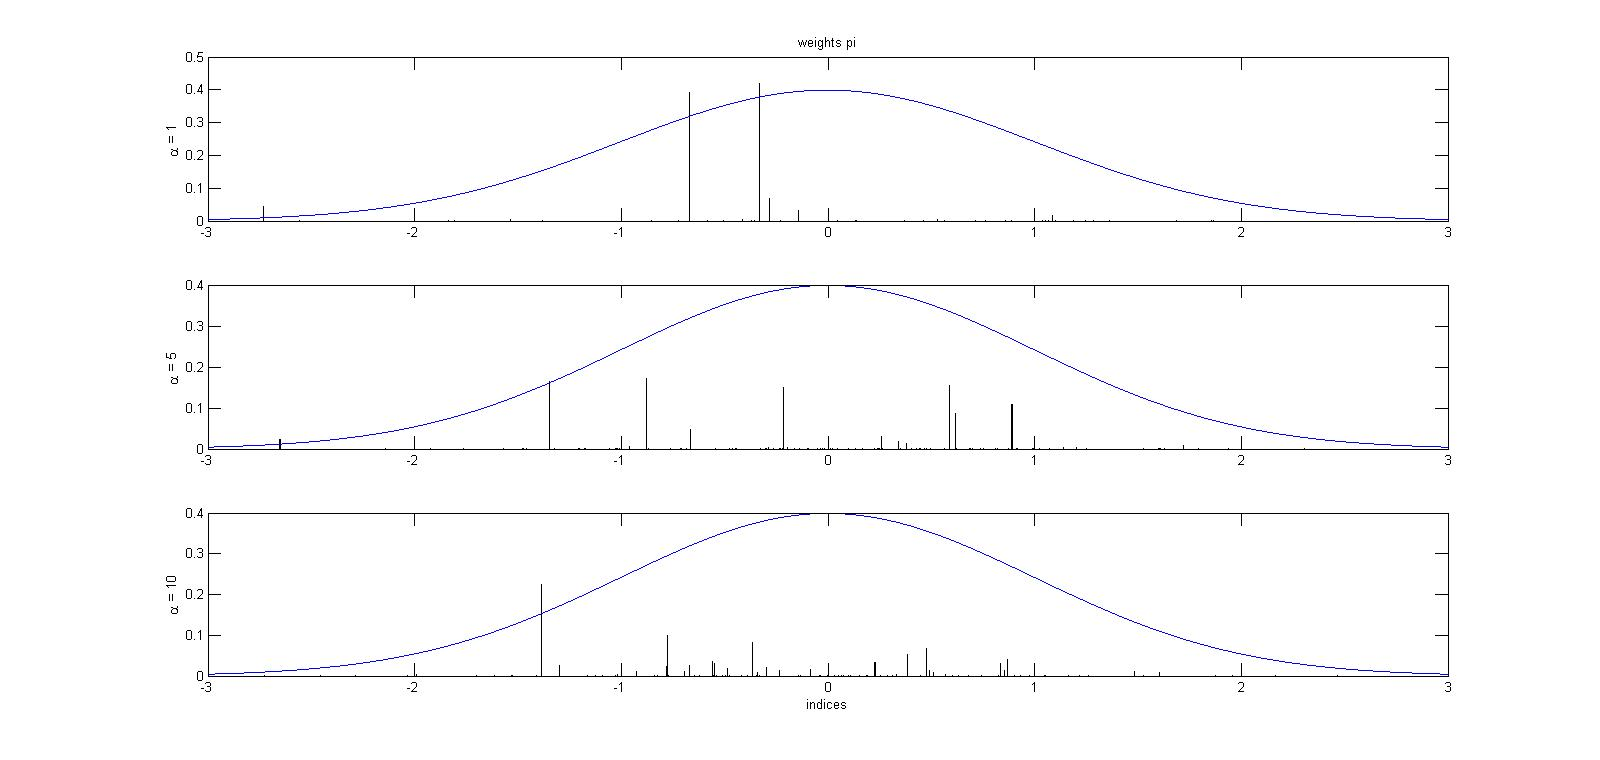
\includegraphics[width=0.91\textwidth]{stickBreakGaus}}
	\caption{The stick breaking process. Every part of the stick represents the number of customers sitting at that specific table in the CRP process. It can be seen that the higher values of $\alpha$ lead to realizations that are closer to the base distribution. It is clear that realizations of a Dirichlet process are discrete distributions.}
	\label{crpGausBase}
\end{figure}

\subsection{Dirichlet process mixture models}

\begin{figure}[!ht]
    \centerline{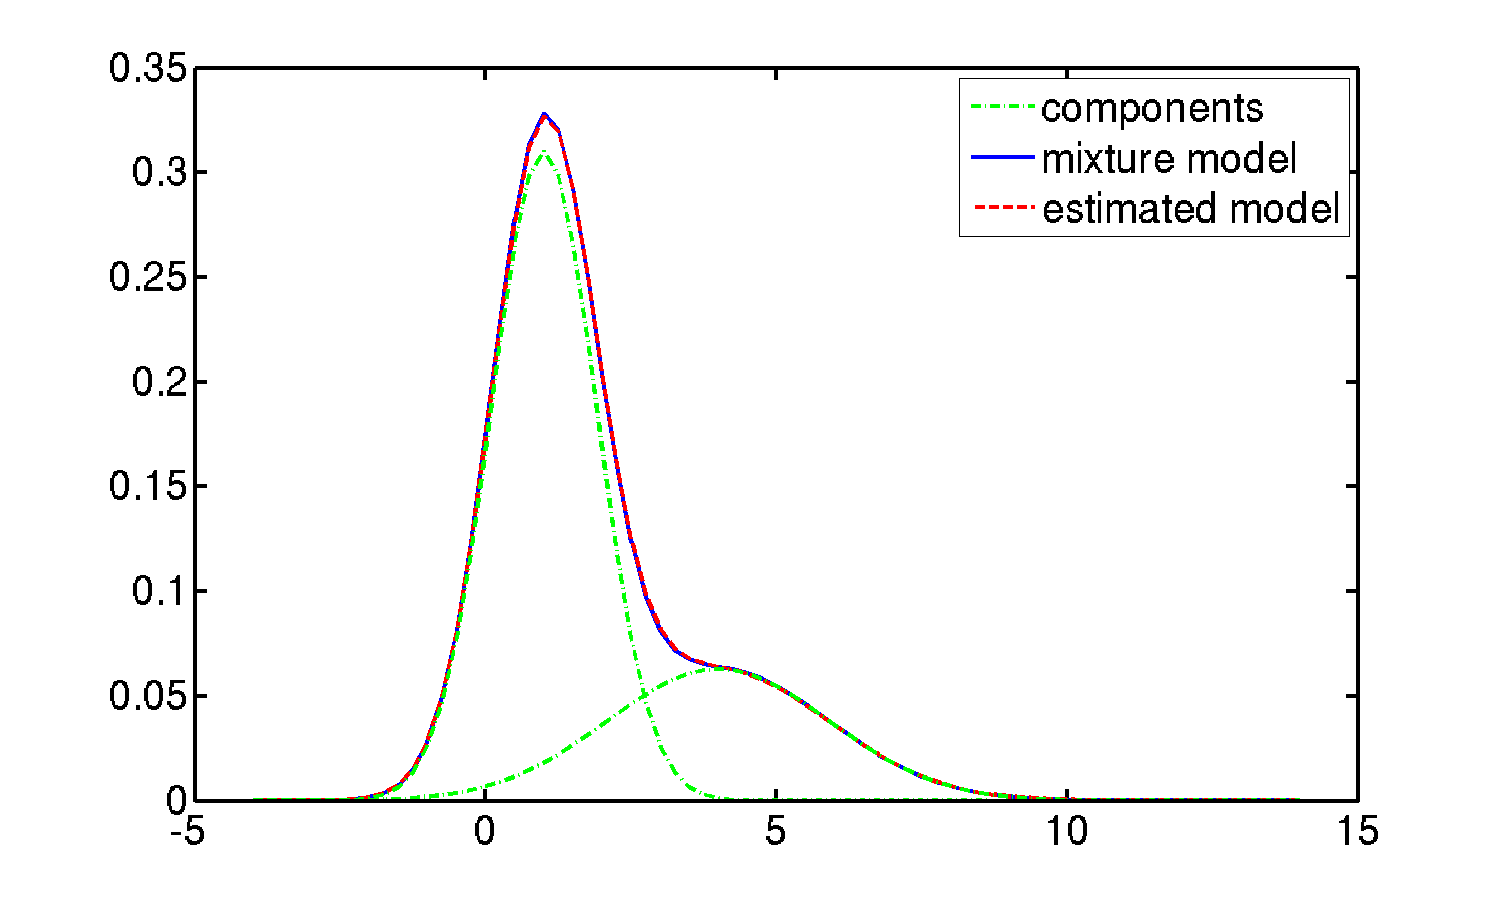
\includegraphics[width=.45\textwidth]{1DGMM}}
	\caption{Mixture model}
	\label{1dGMM}
\end{figure}

One of the most important properties of those objects is that they can serve as a non-parametric prior to mixture models. A typical 1D mixture model that represents data comming from a mixture of two one-dimensional Gaussian distributions is shown in Fig.\ref{1dGMM}.

Mixture models can be considered as the Bayesian approach to clustering, and one of the most important applications of the Dirichlet process is to serve as the non-parametric prior on the parameters of such models. In particular, suppose that observations $x_i$ arise from the following model:
	\begin{equation}
			\theta_i | G \sim G ,
			x_i | \theta_i \sim F(\theta_i )
	\end{equation}

Where $F(\theta_i )$ denotes the distribution of the observation $x_i$ given $\theta_i $. The factors $ \theta_i $ are conditionally independent given G, and the observation $x_i$ is conditionally independent of the other observations given the factor $\theta_i$. When G is distributed according to a Dirichlet process, this model is refered as a Dirichlet process mixture model and its representation is shown in Fig.\ref{mm}. The number of distributions that underlie the data can be mapped to the number of tables within a chinese restaurant process, and the mixing proportions are proportional to the number of people sitting in every table.

Since G can be represented using a stick-breaking construction, the factors $ \theta_i $ take on values $\phi_k$ with probability $\pi_k$. We can denote this using $z_i$ as an indicator variable which takes on positive values and is distributed according to \textbf{$\pi$}. Hence, an equivalent representation of a Dirichlet process mixture model  is given by the following conditional distributions:

	\begin{equation}
		\begin{aligned}
			\centerline{ \textbf{$\pi$} $|$  $ \alpha_0  \sim GEM(\alpha_0 )\ \ \ \ \ \ \ \ \ \ \ \ \ \ \ \   z_i$ $|$ \textbf{$ \pi \sim \pi  $} } \\
			\centerline{$ \phi_k | G_0 \sim G_0 $\ \ \ \ \ \ \ \ \ \ \ \ $x_i | z_i, (\phi )_{k=1}^\infty \sim F(\phi_{z_i}) $  } \\
		\end{aligned}
	\end{equation}

The infinite limit of finite mixture models is taken when we let the number of components into a model to reach infinity. An infinite mixture model assumes that the data come from an infinite number of distributions.

This means that in such models the number of components from which the data are generated can be infinite. In such models it is important to notice in a dataset of size $n$ , the data come from at most n components. This is an important property of infinite mixture models and is exploited when performing posterior inference.

\subsection{Inference}
\begin{wrapfigure}{l}{.3\textwidth}
          \centerline{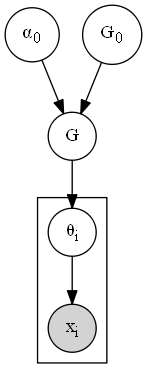
\includegraphics[width=.17\textwidth]{dpmm3}}
	\caption{A Dirichlet process mixture model.}
	\label{mm}
\end{wrapfigure}


Statistical inference is the process of deducing properties of an underlying distribution by analysis of data. Inference can be considered as the inverse procedure presented in the plate in Fig.\ref{mm}; the same graphical process with the arrows facing the opposite direction. Statistical inference techniques can be categorized into 3 families: MCMC, Variational inference and SMC methods. The literature on such methods is extensive and covering it is beyond the scope of this thesis; for the purpose of this thesis an SMC sampler will be defined in detail in the model definition section. 

\subsection{Generalized Polya Urn}


Dirichlet process priors have been widely used in the literature as non-parametric Bayesian tools to estimate the number of clusters in the data\cite{antoniak}. Dependent Dirichlet Processes(DDP) extend those tools by allowing the clusters in the data to vary with some variance over time by introducing dependencies on the data. The DDPs are a natural extension of the Dirichlet processes in domains where data cannot be considered exchangeable. 

A DDP is also known as Generalized Polya Urn\cite{caron}. The most important property of this model is that it randomly deletes partitions of clusters on every iteration. 


This Generalized Polya Urn distribution also has the shorthand notation GPU($\alpha,\rho$) and can be described as follows: At time point $t$ given the clusters at $t-1$ and the data $N_{t-1}$ perform the following: for every cluster and every point within that cluster the point will stay in the cluster or be deleted from it; the probability of a point being deleted from the cluster is proportional to either the size of the cluster or a constant value $\rho <1$\cite{caron}. After the deletion takes place, each point at time $t$ is being assigned to a new cluster $c_{t,n}$  with probability proportional to the size of the cluster at time $t-1$ or assigned to a new cluster with probability proportional to strength parameter $\alpha$ of the prior Dirichlet Process. Cluster sizes are then updated accordingly.


The GPU can be described using the Chinese restaurant process paradigm as follows: At time $t$, customers are seating at several tables in the restaurant. Each customer decides if he/she will remain at table with probability $p$ or definitely leave the table with probability $1-p$. Each customer makes his/her decision and leaves or remains seated. Each table occupied is moved according to the number of customers still occupying the table or is deleted if is currently empty. A new customer then enters the restaurant and either chooses to sit on one of the existing tables with probability proportional to the numer of customers sitting at that specific table or choose table a new with probability to the strength parameter $\alpha$ of the prior Dirichlet process.


\begin{wrapfigure}{l}{.58\textwidth}
    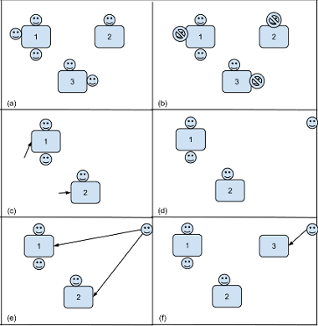
\includegraphics[width=.53\textwidth]{generalPolya2}
    \label{generalPolya}
    \caption{GPU as a function of CRP}
\end{wrapfigure}


Algorithm \ref{gpu:algo} describes the following process: At time step $t$ given cluster assignments at time $t-1$ and data $N_{t-1}$ perform the following: for every cluster and every point within that cluster the point will either stay in the cluster or be deleted from it; the probability of a point being deleted from the cluster is proportional to either the size of the cluster or a constant value $\rho <1$\cite{caron}. Cluster sizes are then modified with respect to the number of points that were deleted from each cluster. After the deletion takes place, each point at time $t$ is being assigned to a new cluster $c_{t,n}$  with probability proportional to the size of the cluster at time $t-1$ after the deletion step or be assigned to a new cluster with probability proportional to strength parameter $\alpha$ of the prior dependent Dirichlet process. Cluster sizes are then updated accordingly.

\begin{algorithm}
  \caption{GPU}\label{GPU}
  \begin{algorithmic}[1]
    \Procedure{GPU}{$t$}

      \For{\texttt{$k = 1,...K_{t-1,N_{t-1}}$}}
	      \State Draw $\Delta s_{t-1}^k \sim Binom(s_{t-1,N_{t-1}}^k, \rho) $ \Comment{Number of elements to delete}
	      \State Set $s_{t,0}^{k} = s_{t-1,N_{t-1}}^{k} -\Delta s_{t-1}^k$
      \EndFor
      \For{\texttt{$n = 1,...N_t$}}
      	    \State Draw $c_{t,n} \sim Cat( \frac{ s_{t,n-1}^{1} }{\alpha + \sum_k s_{t,n-1}^{k} }, \frac{ s_{t,n-1}^{K_{t,n-1}} }{\alpha + \sum_k s_{t,n-1}^{k} } , \frac{ \alpha}{\alpha + \sum_k s_{t,n-1}^{k} }) $
      	    \State If $c_{t,n} \leq K_{t,n-1}\ set:\ s_{t,n}^{c_t,n} = s_{t,n-1}^{c_t,n} + 1 , K_{t,n} = K_{t,n-1}$
      	    \State If $c_{t,n} > K_{t,n-1}\ set:\ s_{t,n}^{c_t,n} = 1 , K_{t,n} = K_{t,n-1} + 1$
      \EndFor
    \EndProcedure
  \end{algorithmic}
  \label{gpu:algo}
\end{algorithm}


\newpage
\section{Model definition}
\label{sec:model}

The model definition section is structured as follows: An introduction to the general pipeline that will serve as the compressed sensor model of the EKF SLAM module is presented first. Every non-trivial component of the pipeline is then analysed in detail with respect to the operations it serves.

\subsection{General pipeline}

\begin{wrapfigure}{l}{0.7\textwidth}
\begin{tabular}{cc}
  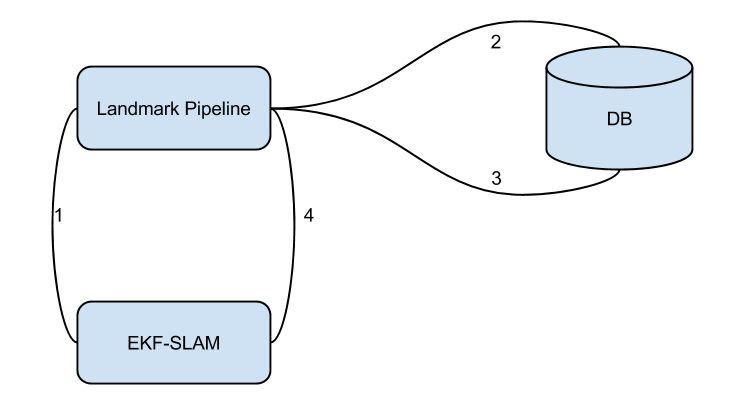
\includegraphics[width=.33\textwidth]{workflowGen} &    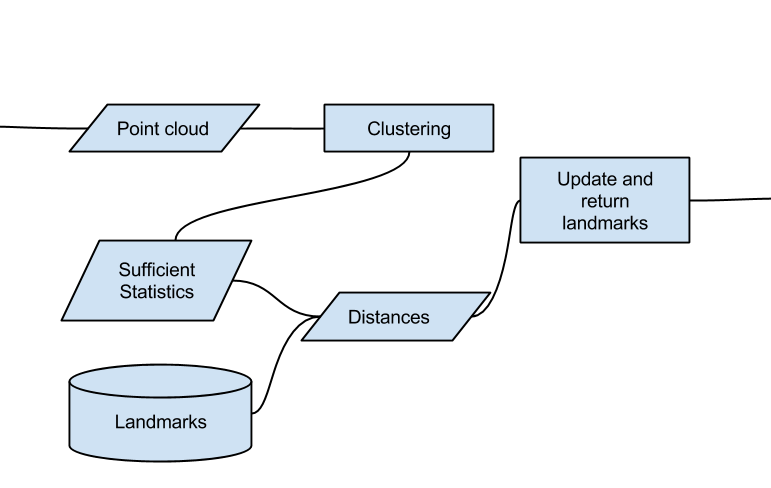
\includegraphics[width=.33\textwidth]{workflowSpec} \\
(a) General pipeline & (b) Landmark pipeline \\[6pt]
\end{tabular}
\caption{General landmark update pipeline}
\label{pipeline}
\end{wrapfigure}


The general flow of operations that defines the basic communication between the pipeline and the EKF module is presented in Fig.~\ref{pipeline}. During step 1 the EKF-SLAM module requests new observation readings given the cloud currently read by the sensors and the position of the robot. The pipeline takes the cloud readings, extracts clusters and returns the landmarks currently being observed while taking into account landmarks that where observed in the past. Landmarks and clusters are identical concepts representing a different layer in the pipeline. More specifically, clusters are output from the sampler and are given as an input of landmarks to the EKF module. Fig.~\ref{pipeline} shows a more detailed view of the computations of the pipeline. The algorithmic procedure shown in Algorithm~\ref{euclid} analytically.


\begin{algorithm}
  \caption{Landmark Layer}\label{euclid}
  \begin{algorithmic}[1]
    \Procedure{getLandmarkIds}{$pC, Landmarks$}
      \State $pCD \gets downsample(pC)$ 
      \State $pCDF \gets extractFeatures(pCD)$
      \State $cls \gets cluster(pCDF)$  
      \For{\texttt{$cls$ as $cl$}}
	      \State $ (sim, landId) \gets calcBestSim(cl, Landmarks) $
			\If{$sim >threshold$}
			   \State $ addLandmarks(landId)$
			\Else 
			   \State $addLandmarks(newID)$
			\EndIf
      \EndFor
      \State \textbf{return} $ landMarkIds$\Comment{Return landmarks}
    \EndProcedure
  \end{algorithmic}
\end{algorithm}


\textbf{Method input:} The method takes as input a pointcloud(pC) as it is currently being read by the kinect sensor.

\textbf{Lines 3-4:} The downsampling and feature extraction are done through the pcl\cite{pcl} library. A voxel grid is used to reduce the dataset size. A leaf size of approximately 3cm produces a good trade-off between precision and speed. The object representation used approach is similar to\cite{objectpointSLAM}. Instead of using the CSHOT descriptor, fpfh\cite{fpfh} histogram is used instead. A fast point feature histogram(fpfh) represents an angular signature between a point and its neighbors. After the fpfh estimation an angular signature of information between a point and its neighbors is acquired. The color signature of the cloud is being encoded with an approach similar to ~\cite{smcddp}. The color spectrum is discretized and what is extracted is the count of different color signatures between a point and its k nearest neighbors. Finally the position of every point is also given as input to the algorithm. The pipeline is presented in figure Fig.~\ref{pcl:mod}. The pipeline outputs a vector of $ \textbf{x} = (x_s, x_c, x_a) $  where $s$ represents a vector of space information, $c$ a vector of colour information and $a$ angular information. 

\begin{figure}[ht!]
  \centering
    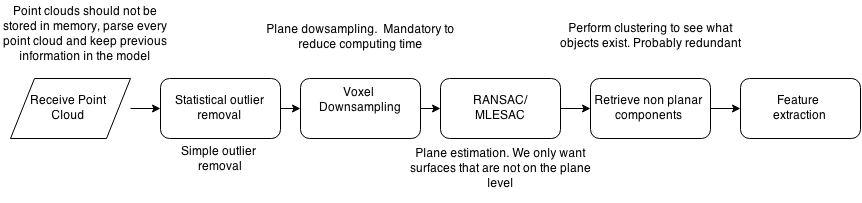
\includegraphics[width=1\textwidth]{Basic}
  \caption{Point cloud modification pipeline.}
  \label{pcl:mod}
\end{figure}

\textbf{Lines 5:} The input of the method is the feature vector for every data point which is calculated in the previous steps. The clustering method is presented in section \ref{smcsampler}. 

\textbf{Lines 6-12:} The correspondence of previously seen landmarks to current observations is computed here. Since the landmarks are distributions, statistical distances can be taken to perform the matching. For every observation, its distances with all the stored landmarks are calculated. calcBestSim returns the cluster with the highest similarity that exists in the database. If the similarity is high enough, correspondence is performed and the landmark is added to the landmark list to be send for update in the EKF, otherwise a new landmark is added and its ID is then added to the list.

\textbf{Lines 13:} The algorithm returns the list of the landmarks the robot currently encounters.

\subsection{The data distribution}
\label{data:dist}

\begin{wrapfigure}{l}{0.35\textwidth}
    \centering
    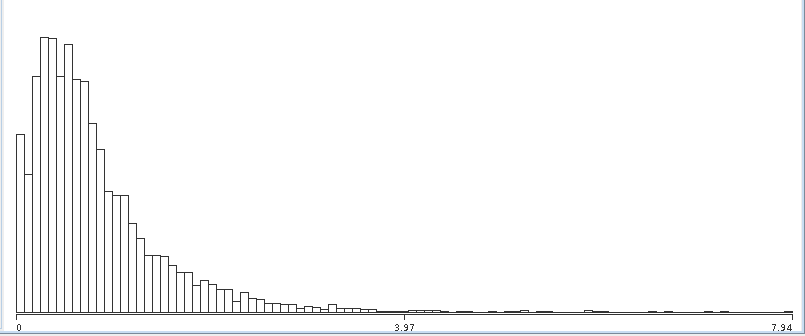
\includegraphics[width=.35\textwidth]{Kullback-Leibler}
    \caption{Exponential trend}
    \label{pcl:kl}
\end{wrapfigure}

Each point $x$ in the cloud is represented as a tuple $x =(x^s, x^a, x^c ) $ where superscript $s$ represents spatial information, $a$ angle information, and $c$ color information. The method those features are extracted is explained in lines 3 and 4 of the general pipeline.

The object model is a mixture of distributions over the data with each object being modeled as F($\theta_t^k$) where $\theta$ represents the parameters of object $k$ at time $t$. More specifically, each set \textbf{X} with $n$ datapoints at time $t$ is distributed as:

\begin{equation}
    \textbf{X}_{t,n} \sim F(\theta_t^k) = Normal(x_{t,n}^s| \mu_t, \Sigma_t) Mult(x_{t,n}^c | \delta_t) Exp(x_{t,n}^a | \lambda_t) 
\end{equation}




Where $Normal$ is a three dimensional normal distribution with mean $\mu$ and covariance $\Sigma$ representing the positional distribution of the data; $Mult$ is a Categorical multinomial distribution with parameter vector $\delta$ representing the color distribution and $Exp$ is an exponential with rate $\lambda$ representing the angle distribution of the data within the cluster. This signature introduces a novel environment abstraction and the purpose of choosing such signature was to have both simple but also informative environment signatures captured by the model. The exponential distribution specifically  was chosen to model angular information after empiric evaluation showed that it would provide a good fit for the angle signature distribution of the data. A typical angle signature distribution is shown in Fig.~\ref{pcl:kl} and the exponential trend of data distances is trivial to distinguish.

Now that the object distribution is defined, the progression of the sufficient statistics at time $t$ given $t-1$ given by:

   \begin{center}
\begin{equation}
    \theta_t^k | \theta_{t-1}^k \sim
   \begin{cases} T (\theta_{t-1}^k) &\mbox{if } k \leq K_{t-1} \\
   G_0 & \mbox{if } k > K_{t-1}. \end{cases}
\end{equation}
   \end{center}
Where $T$ represents the transition kernel of the data given the previous state in the model. The case $ k > K_{t-1} $ represents the creation of a new cluster and $G_0$ is the base distribution of the DDP. In our case, the conjugate priors of the distributions of the data were chosen to model the base distribution. Therefore, $G_0$ is defined as:

\begin{equation}
 G_0(\theta_t^k)  = NiW( \mu_t^k, \Sigma_t^k | \kappa_0, \mu_0, \nu_0, \Lambda_0 ) Dir(\delta_t^k | q_0) Gam( \lambda_t^k | \alpha_0, \beta_0)
 \end{equation}

Where NiW is a Normal inverse Wishart distribution, Dir denotes a Dirichlet distribution, and Gam the Gamma distribution. $ \kappa_0, \mu_0, \nu_0, \Lambda_0, q_0,\alpha_0$ and $\beta_0$ are parameters of the model. The generative process for the Dependent Dirichlet mixture model can be written for each timestep $t$ as:

\noindent\makebox[\linewidth]{\rule{\textwidth}{0.4pt}}
\begin{enumerate}
	\item Draw  $c_t$ $\sim$ $GPU(\alpha, \rho) $
	\item $\forall$  k draw: $ \theta_t^k | \theta_{t-1}^k \sim
	\begin{cases} T (\theta_{t-1}^k) &\mbox{if } k \leq K_{t-1} \\
	G_0 & \mbox{if } k > K_{t-1}. \end{cases}$
	\item $\forall$  point $n$ draw $ x_{t,n} \sim F(\theta_t^{c_t,n})$
\end{enumerate}
\noindent\makebox[\linewidth]{\rule{\textwidth}{0.4pt}}
The transition kernel must satisfy\cite{caron}:

\begin{equation}
\int G_0(\theta_k) T(\theta_t^k | \theta_{t-1}^k) d\theta_{t-1}^k =  G_0(\theta_k)
\end{equation}

The equation means that the invariant distribution must equal its base distribution. A typical way of meeting this restriction and forcing the sampler to converge to the original target density\cite{smc:theory} is to introduce a set of M auxiliary variables \textbf{z} such that:

\begin{equation}
    P(\theta_t^k | \theta_{t-1}^k) =  \int P(\theta_t^k | z_{t}^k)   P(z_t^k| \theta_{t-1}^k) dz_t^k
\end{equation}

The transition kernel of the model can now be sampled by using the following formula:

$\theta_t^k \sim T(\theta_{t-1}^k) = T_2(z_t^k) \circ T_1(\theta_{t-1}^k)$ where:
\begin{equation} \label{eq1}
\begin{split}
    z_{t,1:M}^k  & \sim T_1(\theta_{t-1}^k)\\
 & = Normal(\mu_{t-1}, \Sigma_{t-1}) Mult( \delta_{t-1}) Exp( \lambda_{t-1})
\end{split}
\end{equation}

\begin{equation}
\begin{split}
    \mu_t, \Sigma_t, \delta_t,  \lambda_t & \sim T_2(z_{t,1:M}^k)\\
 & = NiW( \kappa_M, \mu_M, \nu_M, \Lambda_M ) Dir(q_M) Gam(\alpha_M, \beta_M) 
\end{split}
\end{equation}

where $\mu_t, \Sigma_t, \delta_t,  \lambda_t$  are posterior parameters given the auxiliary variables $z$.

\subsection{Sequential monte carlo sampler}
\label{smcsampler}
Sequential Monte Carlo(SMC) samplers for Dirichlet process mixture models where introduced by Doucet et al.~\cite{doucet} and serve as fast alternative to Markov Chain Monte Carlo and Variational Inference methods of performing posterior inference. SMC samplers have known strengths and weaknesses and are a good fit for the problem at hand, as their main theoretical disadvantage, the particle degradation is hard to occur at the minimal time horizon that the sampler is being used. We can now define the SMC sampler that will be used to perform inference on our model as follows:

\begin{algorithm}[ht!]
  \caption{SMC for DDPM}\label{SMC}
  \begin{algorithmic}[1]
	\State \textbf{Input:} Points \{$x_{1,1:N_t}, ..., x_{T,1:N_t}$\}
	\State \textbf{Output:} Clusters that best fit input data
	\For{$t = 1,...T$} 
			\For{$ l = 1,...L$} 
							\For{$ i = 1,...S$} 
								\State Sample $(c_t)^{(l)} \sim Q_1$  
								\State Sample $(\theta^k ) \sim Q_2$
						    \EndFor		
		    \For{$ k = 1,...K$} 
			   \State Sample $\Delta s_{t-1}^k \sim Binom( (s_{t-1,N_{t-1}}^k)^{(l)}, \rho) $ 
		       \State Set $s_{t,0}^{k} = s_{t-1,N_{t-1}}^{k} -\Delta s_{t-1}^k$
   		       \State Sample $( (z_{t+1}^k)^{(l)} ) \sim T_1((\theta_t^k))^{(l)} $
		    \EndFor
		 	\State compute particle weights $w_t^l$
		    \EndFor
    \State Normalize weights and resample
    \EndFor
  \end{algorithmic}
\end{algorithm}

The process  presented in Algorithm \ref{SMC} can be described as follows:
For every time step $T$ for every particle $L$ and for every sample $S$, sample cluster indexes $c_t^{(l)}$ from the proposal distribution $Q_1$ and sufficient statistics from proposal distribution $Q_2$ as they are defined in section \ref{gibbsUpd}. After clusters assignments and sufficient statistics are sampled for all the samples and particles, perform the deletion step of the DDP and sample auxiliary variables with from the transition kernel of the elements that stayed in the clusters after the deletion steps. Compute the weights and perform the resampling. 

\subsubsection{Gibbs updates}
\label{gibbsUpd}
The proposal distribution $Q_1$ is the probability of an assignment $c_{t,n}$ given cluster sizes, parameters and concentration $\alpha$. Formally $Q_1$ can be written as:
\begin{equation} \label{Gibbs}
 Q_1(c_{t,n} | s_{t,n}^k, \theta_t^k, \alpha) \propto Cat( s_{t,n}^1,...s_{t,n}^K, \alpha ) \times
 	\begin{cases} 
 	F(x_{t,n} | \theta_t^{c_t} )  &\mbox{if } k \leq K_{t-1} \\
 	\int P(x_{t,n} | \theta_t )G_0(\theta) d\theta & \mbox{if } k > K_{t-1}. \end{cases}
\end{equation}
Where $c_{t,n}$ represents cluster $c$ of point $n$ at time $t$, $s$ represents cluster sizes. The integral represents the posterior predictive distribution of the cluster times the base distribution with the parameters integrated out. More specifically, the analytic expression of the integral is:


\begin{equation} \label{Q1}
	\begin{split}
		 	\int P(x_{t,n} | \theta_t )G_0(\theta) d\theta =
		 	\int Normal(x_{t,n}^s| \mu_t, \Sigma_t) Mult(x_{t,n}^c | \delta_t) Exp(x_{t,n}^a | \lambda_t) \times  \\ NiW( \mu_t, \Sigma_t | \kappa_0, \mu_0, \nu_0, \Lambda_0 ) Dir(\delta_t | q_0) Gam( \lambda_t | \alpha_0, \beta_0)  d\theta  \\
			= \int Normal(x_{t,n}^s| \mu_t, \Sigma_t) \times NiW( \mu_t, \Sigma_t | \kappa_0, \mu_0, \nu_0, \Lambda_0 )\\
			 Mult(x_{t,n}^c | \delta_t) \times Dir(\delta_t | q_0) \\
			 Exp(x_{t,n}^a | \lambda_t) \times Gam( \lambda_t | \alpha_0, \beta_0)  d\theta  \\
		 	= t_{\nu_0-1}( x_{t,n}^s | \mu_0, \frac{\Lambda_0(\kappa_0+1)}{\kappa_0(\nu_0-1)}) \times \prod_{j=1}^V \frac{\Gamma(x_{t,n}^c)}{\Gamma(q_0)} \times \\ \frac{\Gamma(\sum_{j=1}^V q_0)}{\Gamma(\sum_{j=1}^V x_{t,n}^c)} \times Lomax(\alpha_0 + s_{t,n}^c, \beta_0 \sum_{j=1}^V x_{t,n}^c)
 	\end{split}
\end{equation}

Where $t$ represents student's t-distribution with $\nu$ degrees of freedom, Lo
max represents Lomax distribution with shape and scale, $\alpha$ and $\beta$ repsectively and the rest represent a Dirichlet-Multinomial(aka DirMul) distribution. The formulas of the posterior predictive distributions can be found in the literature with \cite{compendium} being a good example. 

The integration is easy to calculate due to two basic assumptions on the data. Firstly, the object distribution and the base distribution are build such a way that their respective counterparts consist of conjugate distributions. Since literature on calculating the posterior predictive distribution of two distribution with the parameters of the distribution intergrated out, finding the result is a matter of finding the correct formula\cite{compendium}. Secondly, due to that every pair of prior distribution along with its respective likelihood are independent from every other pair given the parameters $\theta$ it is easy to calculate this integral in closed form.

The conjugacy of the base and prior distribution also allow for an easy sampling formula for proposal distribution $Q_2$ which is of the form: 


\begin{equation} \label{Q_2}
\begin{split}
Q_2(\theta_t^k | \theta_{t-1}^k , x_t^k, z_t^k) \propto F( x_t^k | \theta_k) \times T_2(\theta_t^k | z_t^k) \\
= NiW( \mu_t^k, \Sigma_t^k | \kappa_n, \mu_n, \nu_n, \Lambda_n ) Dir(\delta_t^k | q_n) Gam(\lambda_t^k | \alpha_n, \beta_n)
\end{split}
\end{equation}

With:

\begin{equation} \label{udpates}
\begin{split}
\kappa_n = \kappa_0 + N ,
\nu_n = \nu_0 + N ,
\mu_n = \frac{\kappa_0}{\kappa_0 + N} \mu_0 +  \frac{N}{\kappa_0 + N} \overline{x}^s\\
\Lambda_n = \Lambda_0 + s_{x}^s,
q_N = q_0 +  \sum_n x_i^c,
\alpha_n = \alpha_0 +  N,
\beta_n = \beta_0 +  \sum_n x_i^a
\end{split}
\end{equation}


Where $\overline{x}$ defines the sample mean for the elements assigned at cluster $c$, $s_{x}$ the sample variance and $N$ denotes the number of observations\cite{conjugate}.

\subsubsection{Weight updates}

Finally, the weight update step is defined as follows: On every time step $t$ the weight of particle $l$ is calculated as:

\begin{equation}
w_t^{(l)} = \frac {P(c_t^{(l)} , \theta_t^{(l)}, x_t| 	\theta_{t-1} )}{P(c_t^{(l)} , \theta_t^{(l)}| 	\theta_{t-1} )}
\end{equation}

Using Bayes rule, the numerator can be written as:

\begin{equation}
	P(x_t , | c_t^{(l)} , \theta_t^{(l)} \theta_{t-1} ) \times P(c_t^{(l)} , \theta_t^{(l)}|  \theta_{t-1} )
\end{equation}

Which can be calculated using equations $Q_2$ and $Q_1$ for the first and second part respectively. After the particle weights are normalized particles are drawn with probability proportional to their weights.

\subsection{Decision Layer}

Once the points of the current iteration are grouped, the clusters that were infered are passed as input to the decision layer. The decision layer calculates the similarity of the current clusters to past ones; if the similarity is high enough the clusters are considered to be part of the same landmark. To do that, distance measures between the stored clusters and the ones that are inferred at the current iteration of the algorithm must be defined. Distances between distributions are called divergences and a large amount of literature on divergences exists.

Every cluster consists of a three part distribution as it was defined in section \ref{data:dist}. To define a distance measure between cluster, individual distances between all the distribution parts will be defined. More specifically let $l$ be the distribution of a cluster encountered in the past and $o$ the distribution of a currently observed cluster. $l$ and $o$ can be decomposed into 3 parts: $l_G$,$l_C$,$l_E$ where G,C and E stand for Gaussian, Categorical and Exponential respectively. With that notation the distances between those distributions can be defined. For each individual landmark distribution $l$ and observation distribution $o$ the distances computed where the following: A Wesserstein($l_G,o_G$), a Kullback-Leibler($l_G,o_G$), a SquaredHellinger($l_E,o_E$),a Kullback-Leibler($l_E,o_E$) and  Kullback-Leibler($l_C,o_C$).

With that in mind the distance between every distribution can be transposed to a vector where each element represents a specific distance between the two distributions. That way, deciding if a cluster is part of a landmark that has been encountered before is now a problem of finding the optimal decision boundary given the distances at hand. For the purposes of this thesis, the decision boundary of an observation being a landmark or not was chosen by empiric evaluation of the landmarks. It is of course possible to learn the optimal decision boundary but due to time restrictions a simpler decision making approach was chosen instead.

\subsection{Complexity}
\label{subsec:complexity}
The complexity can be decomposed into three parts. The cloud downsampling, the clustering and the decision making process.
$$
O(total) = O(filter) + O(cluster) + O(decision)
$$
\textbf{Downsampling}: The complexity of the cloud downsampling pipeline can be decomposed to the one of its components. This means that the decomposed complexity is defined as follows:
$$O(filter) = O(Downsampling + Stat\ Removal + RANSAC+ FPFH + Color\ est) $$

Voxel downsampling searches for neighbors within a distance defined by the user and keeps an average value that equally represents the cloud. Since the operation involves searching for neighbors of a point, and since search operations take $O(log\ n)$ time where N is the number of points within the cloud, the complexity of voxelGrid downsampling is $O(k log n)$ where $k$ is the number of neighbors and $n$ the number of points in the cloud. 
Statistial outlier removal searches for k nearest neigbhors and removes those whose deviation is passed a certain threshold. Given that search operations take $O(log\ n)$, for k neighbors, the complexity is $O(k\ log\ n)$. The same assumption regarding the averaging computations is done here.
A high amount of research has been done regarding the optimal complexity of RANSAC~\cite{RANSAC}. RANSAC has a complexity of $ O(k+ m_s*N)$ where k is the maximum amount of iterations defined by the user, $m_s$ the average number of models per sample $N$ the number of data points.
FPFH operations have a complexity of $O(nk)$ as given in~\cite{fpfh}.
Finally, for the operation of color estimation, the k nearest neighbors are chosen and some constant operation is performed on them. The complexity here is similar to Statistical outlier removal since operations after the search are assumed to take take $O(1)$ time. The complexity for color estimation then becomes $O(k\ log\ n)$ where $k$ is the number of neighbors, $n$ the number of points. 

The downsampling pipeline has a total complexity of:
\begin{equation} \label{Q_filt}
O(filter) = O(k_{0}\ log\ n_{init} + k_{1}\ log\ n_{1} + k_{2}+ m_s*n_{2} + n_{3}k_{3} + k_{4}\ log\ n_{3} )
\end{equation}

The different $k$ indexes represent the number of neighbors defined for every operation. The $n$ represents the number of points used as input. Using the notation of equation \ref{Q_filt}, $n_{init}$ defines the whole cloud, $n_1$ the cloud after operation 1, $n_2$ the cloud after operations 2 and so on.

\textbf{Clustering}: The complexity of the SMC sampler is defined in \cite{smcddp} as $O(TLKSN)$ where $T$ defines the time frames, $L$ the number of particles, $K$ the number of clusters, $S$ the number of samples, and $N$ the size of the dataset. 

$$
O(cluster) = O(TKLSN)
$$

\textbf{Decision making}: The decision making takes $ O(\kappa * l^2) $ computational time where $\kappa$ defines the number of clusters output by the sampler and $l$ the number of landmarks currently stored in the database. This number can be further reduced by taking for example only landmarks that are nearby the cluster, but optimizing the decision making performance is outside the scope of this thesis.


Finally, with some notation abuse, the final complexity of the method can then be defined as:

\begin{equation} \label{complexity}
\begin{split}
O(filter) + O(cluster) + O(decision) = \\
O(k_{0}logn_{0} + k_{1}logn_{1} + O(k_{2}(t_M)+ m_s*n_{2}) + n_{3}k_{3} + k_{4}logn_{3} ) + O(LKSn_3) + O(\kappa * l^2)=\\
O(k_{0}logn_{0} + k_{1}logn_{1} + k_{2}(t_M)+ m_s*n_{2} + n_{3}k_{3} + k_{4}logn_{3} + LKSn_3 + \kappa * l^2)
\end{split}
\end{equation}

The complexity as defined in equation~\ref{complexity} depends on the initial reduction of the voxel downsampling. As the voxel leaf size parameter decreases and the downsampling outputs a larger cloud, the precision as well as the computing time of the method increases. Since in this thesis the research was directed towards online SLAM methods, the leaf size was modified so that the cloud the time requirements for online landmark tracking were met.

\subsection{Landmark size}


The basic block of this algorithm is a cluster containing an environment signature. In order to be able to compute how scalable the method is, the size a single cluster requires to be stored will be calculated. Each cluster is represented by the paramters of the distributions in contains; these values are passed in a single row in a database\cite{sqlite}. According to the database manual the maximum number of memory a single landmark can require is 260 bytes. Calculations in the results section are done using 260 bytes as a unit cost of the method. 

\newpage
\section{Results}
\label{sec:results}

The results of the method will be presented and analysed in this section. A simple dataset will first be presented to introduce the reader to the environment signature the sampler outputs. The decision layer subsection introduces the behaviour of the decision boundary of the sampler with respect to the color and position of the clusters infered. The pipeline is then used as a sensor model in the EKF-SLAM experiments section and the results of the mapping are presented and analysed. Finally, to address the research questions that were formulated in the introduction the method was tested for its speed and memory requirements.


\subsection{Simple datasets}

In this section the algorithm will be tested against a simple dataset. That will make easier the conceptual extension to more complex clouds that will be used when mapping the environment. In order to test the sampling as well as the decision layer of the algorithm, a simple dataset provided by the pcl\cite{pcl} library was used. More specifically, a cloud consisting of two milk cartridges(Fig. \ref{pcl:clust}(a)) with different colors and poses was used. 

\begin{figure}
\begin{tabular}{c}
  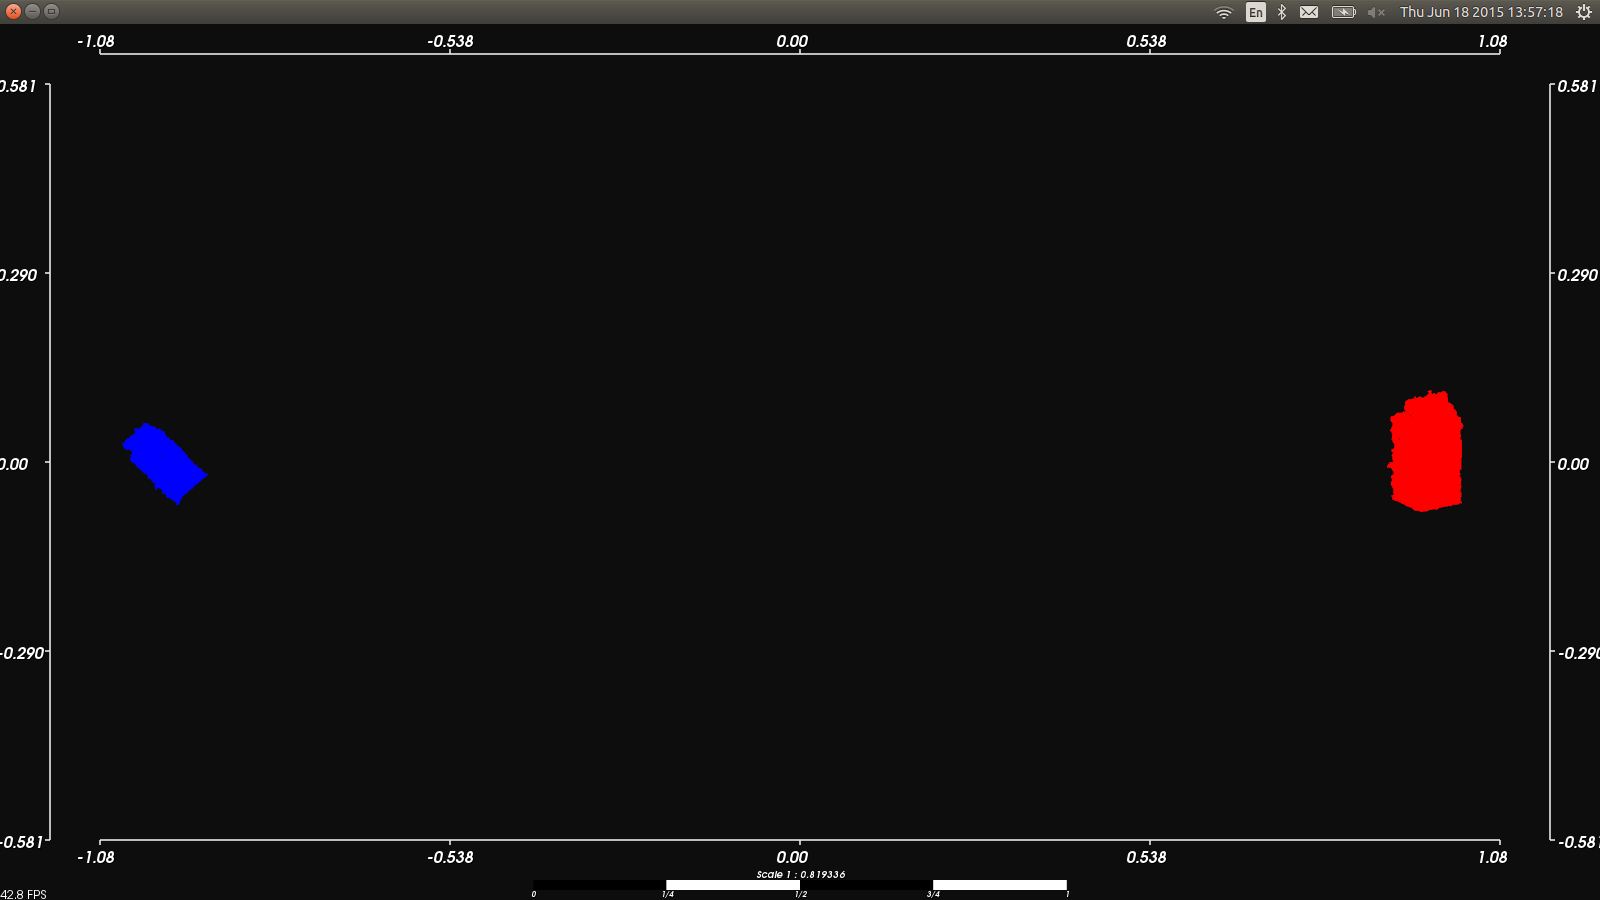
\includegraphics[width=1\textwidth]{clusterings/initialData} \\
  (a) Initial cloud. This cloud is given as input to the downsampling pipeline.  \\
   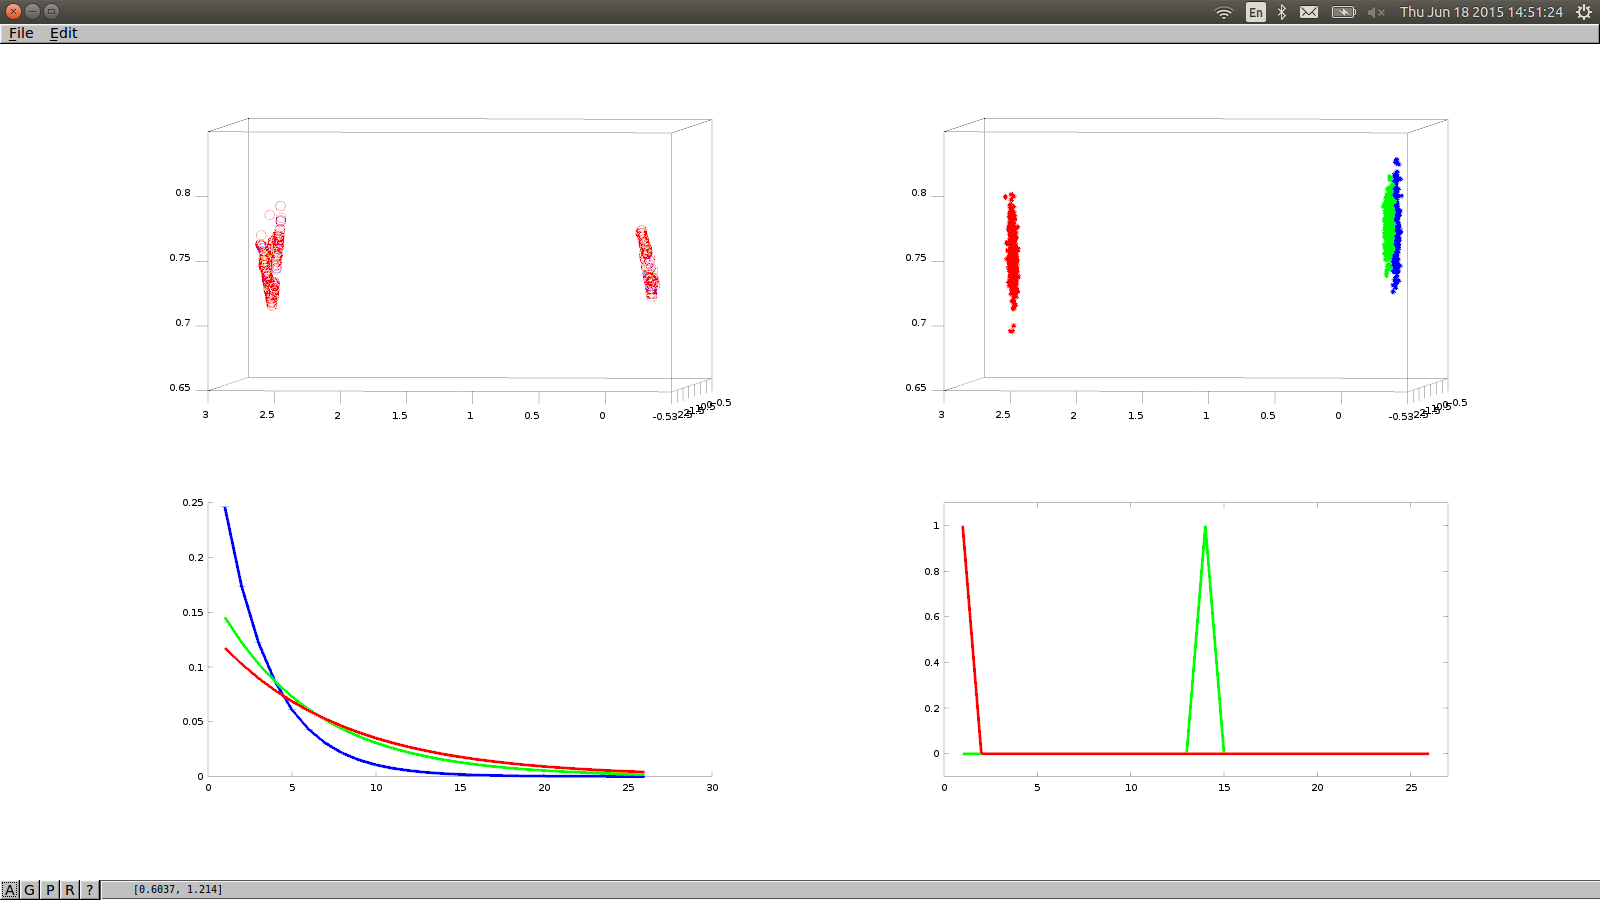
\includegraphics[width=1\textwidth]{clusterings/colorcodedDistributions} \\
 (b) Downsampling and clustering results. Top left picture shows the cloud that is given as input\\
 to the sampler. Top right(Gaussian) and bottom(Exponential, Categorical) subfigures show the \\
 distributions infered from the data.  The different clusters signatures  are color coded. \\
 Blue and red signatures override completely since they carry identical color signatures.\\
 \end{tabular}
\caption{Initial data along with the distributions infered }
  \label{pcl:clust}
\end{figure}


\begin{figure}
\begin{tabular}{c}
  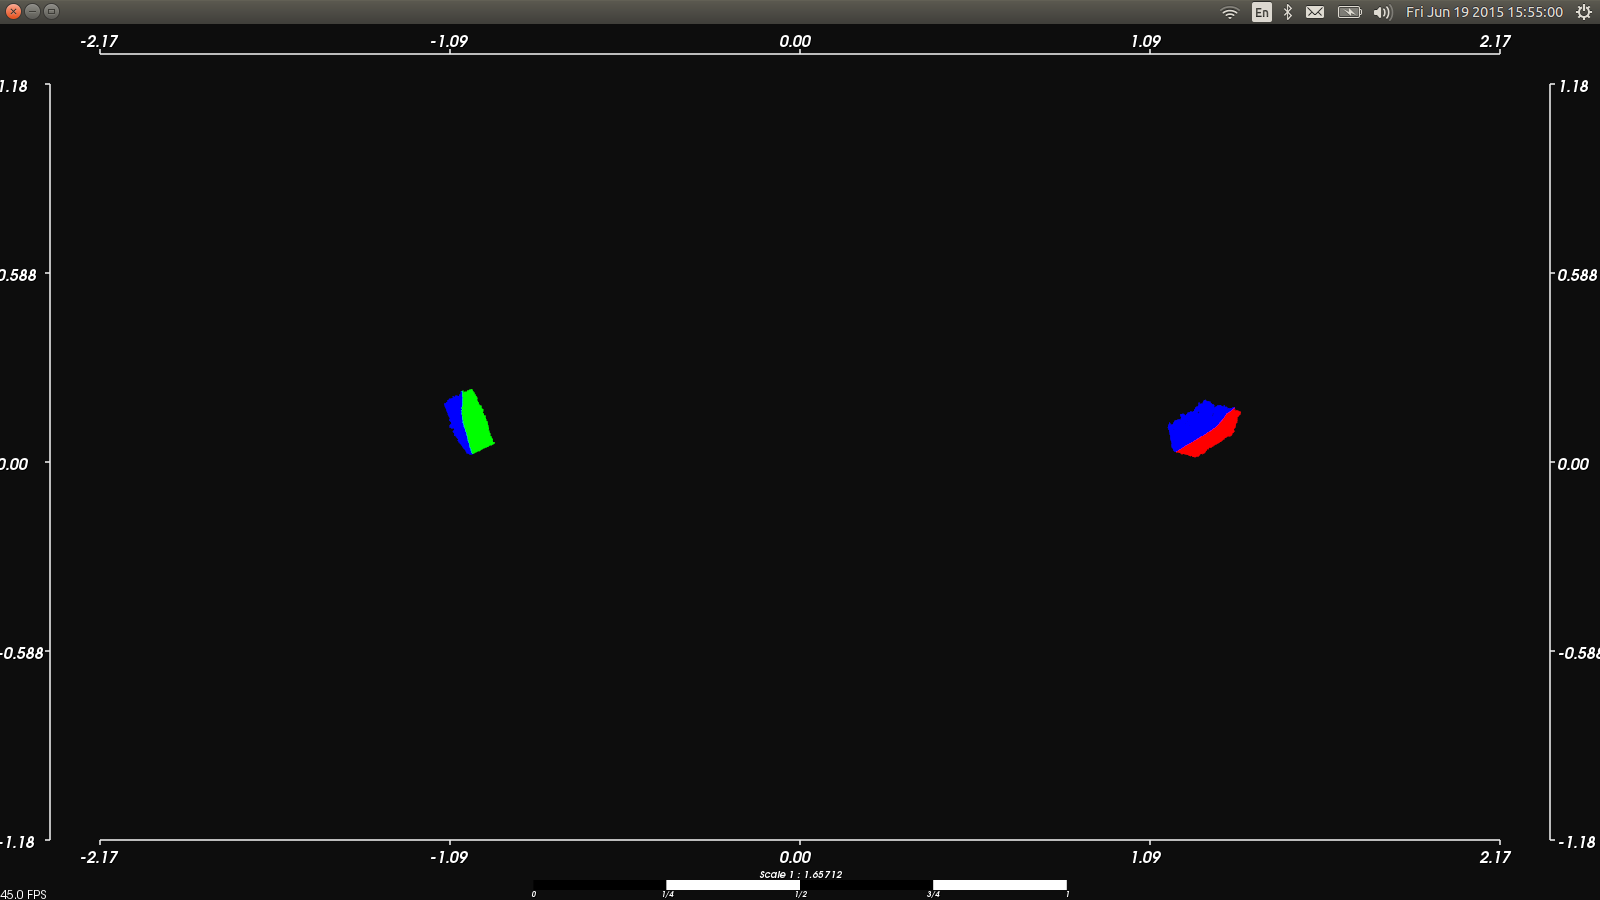
\includegraphics[width=1\textwidth]{clusterings/coloursSource} \\
  (a) Initial cloud. This cloud is given as input to the downsampling pipeline.    \\
   Notice the more complicated colors the milk catridges have. \\
   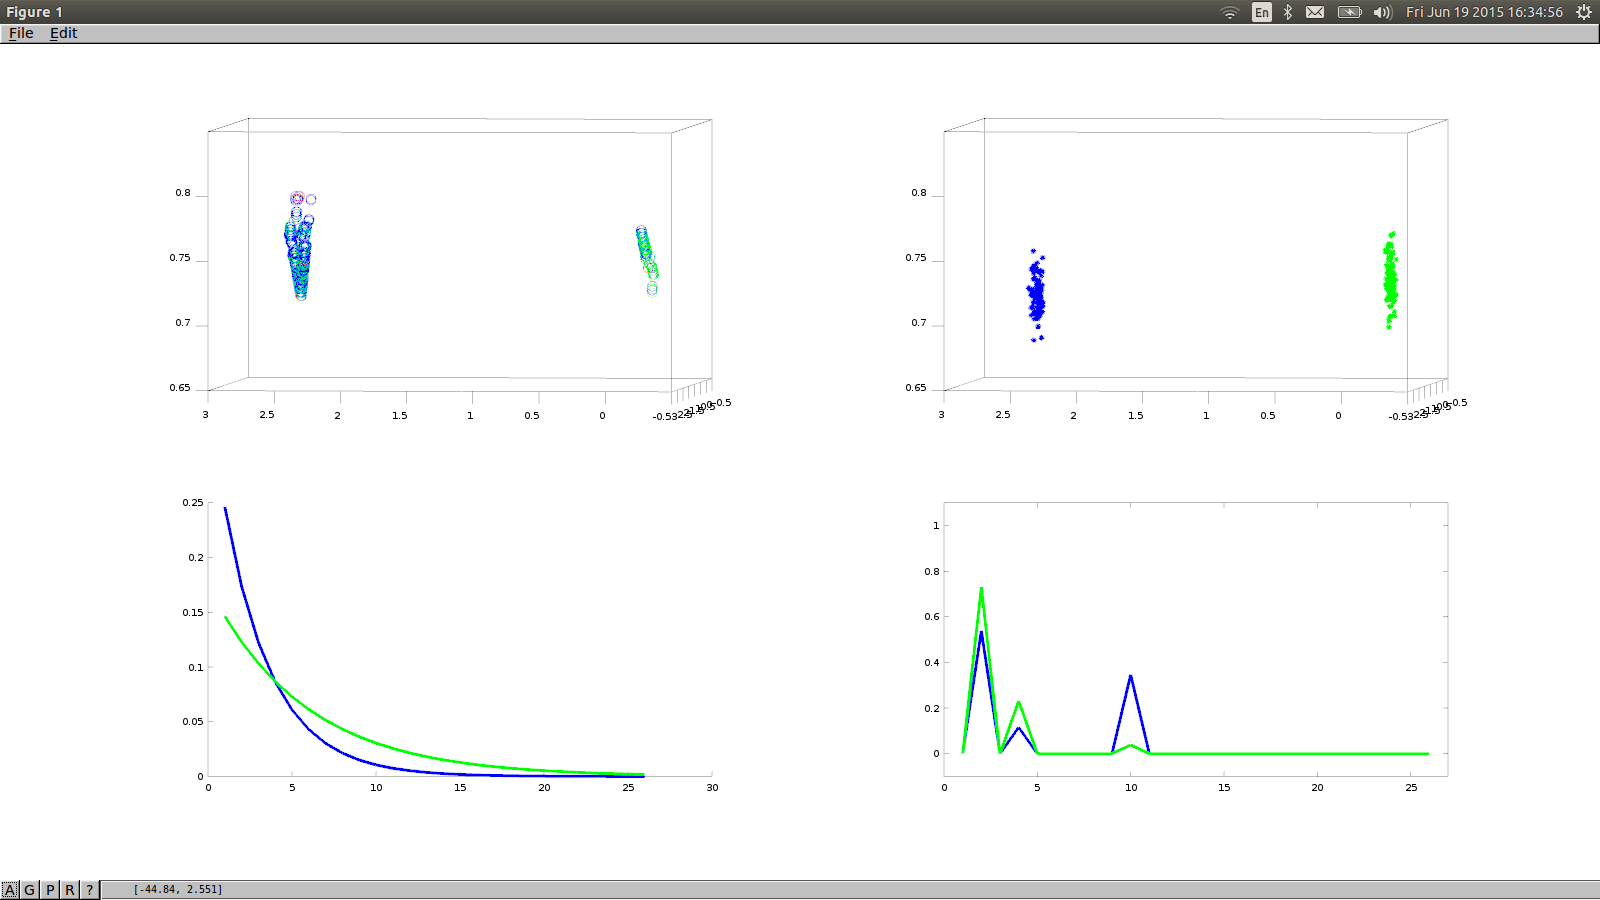
\includegraphics[width=1\textwidth]{clusterings/coloursCorrect} \\
 (b) Downsampling and clustering results. Top left picture shows the cloud that is given as input\\
 to the sampler. Top right(Gaussian) and bottom(Exponential, Categorical) subfigures show the \\
 distributions infered from the data. The colors in the distribution signatures display \\
 the different clusters infered.\end{tabular}
\caption{More complicated color distributions}
  \label{pcl:clust2}
\end{figure}

The cloud was parsed from a cloud file(.pcd) and was given as input to the downsampling and feature extraction pipeline. The reduced cloud(top left Fig.\ref{pcl:clust}(b)) was then passed as input to the sampler and the clustering results are shown in Fig.\ref{pcl:clust}(b). The downsampling reduces a cloud of 27408 points in 4493 producing a significantly smaller cloud; this cloud along with all feature information calculated are given as input to the sampler. The sampler outputs a mixture of distributions that fits the input data. The clustering output is shown in Fig.\ref{pcl:clust}(b) with the top right being the Gaussian distributions inferred, bottom left the exponential and bottom right the categorical representing the color information of the cloud. The sampler outputs 3 clusters for the data and it can be seen that the change in angular information of the box leads the sampler to assign two distributions in the left milk box cloud. The color information is captured correctly in the structures and that was expected since the data had distinct colour signatures.

\begin{table}[!ht]
\begin{center} 
    \begin{tabular}{|C|C|C|C|C|C|}
    \hline
    \multicolumn{6}{|l|}{\centerline{LandmarkId 1}} \\
    \hline
     LandmarkId & GausKL & GausWes & ExpKL & ExpSqHell & CatKL \\
	 \hline
 	 2&0.0115821&53.5171&1.20726&0.319589&0 \\
 	 \hline
	 3&13.5579&22449.9&1.56956&0.376699&13.8155 \\
	 \hline
    \multicolumn{6}{|l|}{\centerline{LandmakId 2}} \\
    \hline
	 1&0.0115821&20.1454&1.7215&0.319589&0 \\
	\hline
	3&12.8379&21458.6&0.474719&0.449769&13.8155 \\
	 \hline
    \multicolumn{6}{|l|}{\centerline{LandmarkId 3}} \\
    \hline
	 1&13.5579&31191.5&2.55205&0.376699&13.8155\\
	 \hline
     2&12.8379&65013.8&0.53855&0.449769&13.8155\\
	 \hline
	 \end{tabular}    
     \label{distancesofclusters}
\end{center}
\caption{Distances between the distributions infered in Fig.\ref{pcl:clust}}
\end{table}


After the structure is clustered, distances between the elements can be calculated. Table \ref{distancesofclusters} shows the distances between every cluster shown in Fig.\ref{pcl:clust}. It can be seen that the first two landmarks have small distances in their Gaussian counterparts since they represent nearby areas and objects in the cloud that are very far apart. The angular distances are represented by the ExpKL and ExpSqHell rows. The distinct colors of the milk boxes are correctly captured in their respective cluster signatures. The calculated distances are then given to the decision layer to caclulate if the clusters currently calculated are part of landmarks previously encountered.
An example with more complex color signatures is shown in Fig.\ref{pcl:clust2}. The clouds are now given a mixture of colors and this is passed to the color signature inferred on every cluster in Fig.\ref{pcl:clust2}. In this case the sampler outputs 2 clusters and the color signatures capture the more complex color signatures as well as the expected overlap correctly. 

\subsection{Expressivensess and decision layer}

Are such representations rich enough to be used as references points when performing SLAM?
To test the expressive strength of the representation, experiments were performed to test how the representation in combination with the decision layer differentiated over different objects in the cloud. 
The decision boundary of the pipeline can be decomposed into three basic parts; a positional, a color and an angular boundary. Fig.\ref{pip:bounds} shows the behavior of the decision layer with respect to the Gaussian(positional) and Categorical(color) parts. 
    
\begin{figure}

\begin{tabular}{cc}
  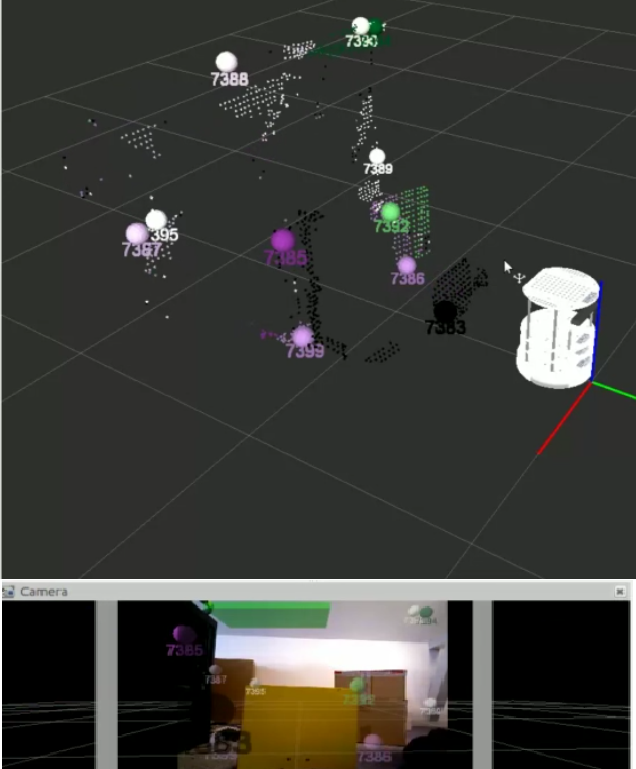
\includegraphics[width=.45\textwidth]{colorBound5} &   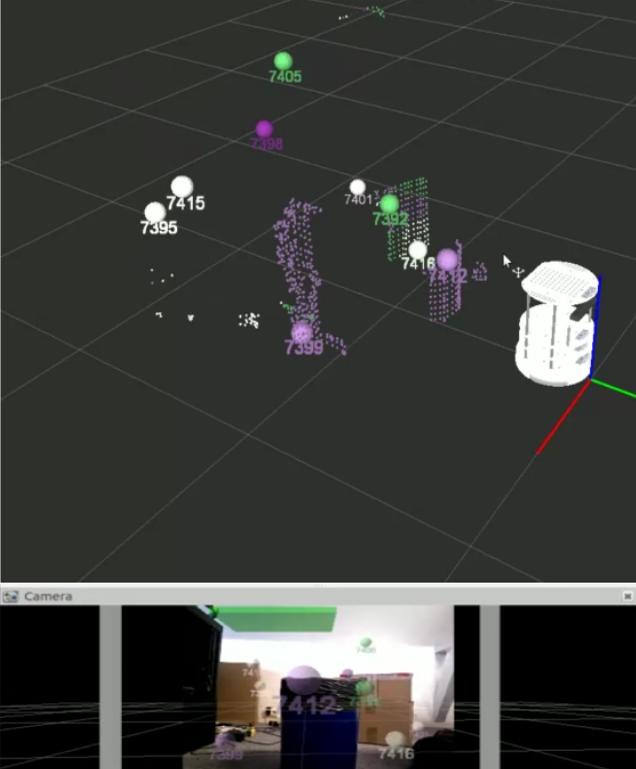
\includegraphics[width=.45\textwidth]{colorBound6} \\
(a) Yellow Folder assignment  & (b) Blue trashcan assignment \\[6pt]
	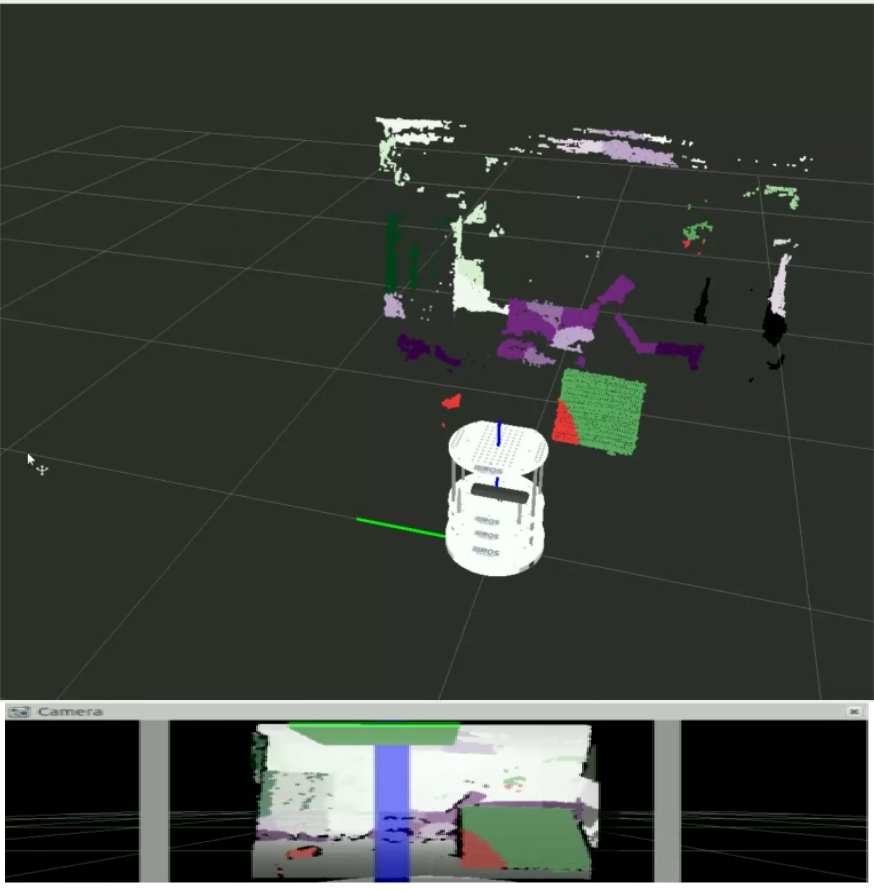
\includegraphics[width=.45\textwidth]{posBound5} &   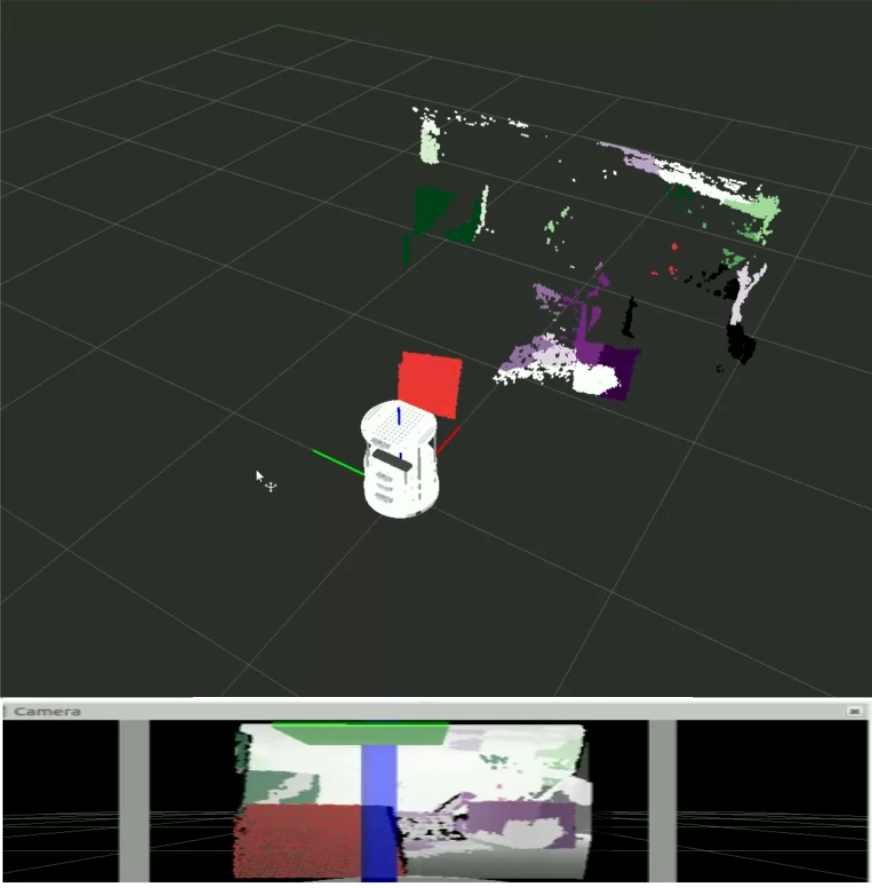
\includegraphics[width=.45\textwidth]{posBound6} \\
(c) Folder initial  & (d) Folder moved \\[6pt]
\end{tabular}
\caption{The colour and position boundary is displayed in these pictures}
  \label{pip:bounds}
\end{figure}

In the first picture of Fig.\ref{pip:bounds} the yellow folder along with some of its environment to the left are being assigned to landmark with id 7386(color coded black). The folder is then removed and a blue trashcan is put in its place. The folder and the trashcan are similar in size; due to that their Gaussian counterparts will not have large distances. Their main difference lies in the color signature they carry. Since the distance in their color is substantial, a new landmark with id 7412(color coded purple) is created to capture the change in the signature of the environment at that place of the map. The different landmark assigned to the cluster can be seen the second picture in Fig.\ref{pip:bounds}. The positional decision boundary is displayed in the third and fourth picture of Fig.\ref{pip:bounds}. In the initial position the yellow folder is assigned to the green landmark of the cloud. As the object is moved a different position in the cloud, it is being assigned to a different cluster. The reason the cluster is assigned to multiple landmarks is due to the fact that the folder is decomposed to several clusters and each one of them is being assigned to a different part of the cloud with respect to their position. This can be seen in the fourth picture of Fig.\ref{pip:bounds} where the bottom left of the folder is being assigned to the red cluster.

The exponential part of the distribution is responsible for the angle signature elements within a cluster carry. Having a very strict limit in the angle distribution can lead to very small clusters and subsequently to a high amount of landmarks within the data. Practical evaluation has shown that using an angle limit that is close to the average distance between angle signatures produces stable results and reasonably sized landmarks in the cloud.

\subsection{EKF-SLAM experiments}


\begin{figure}
  \centering
    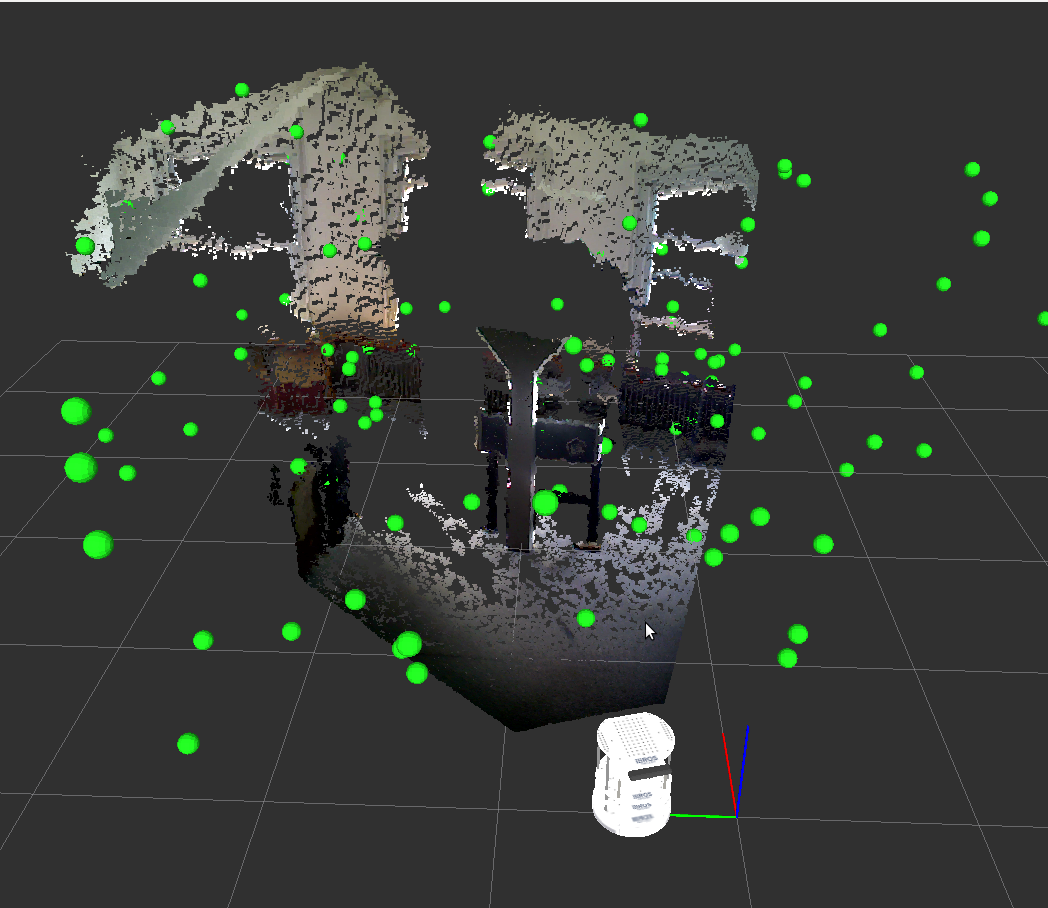
\includegraphics[width=.5\textwidth]{SLAM110landmarks2}
    \caption{SLAM session using the pipeline. The pipeline is used as the sensor model of an EKF-SLAM module. The readings of a kinect mounted on a turtlebot are downsampled and clustered. Current readings are either being matched to past readings giving old landmarks or being used to create new landmarks if no similar past environment sigantures exist. Landmarks are represented with yellow spheres. }
  \label{SLAM}
\end{figure}


The pipeline was used in real life scenarios as a sensor model in a Landmark based EKF SLAM algorithm and was further tested for its speed and memory requirements. Fig.\ref{SLAM} shows an end result of a SLAM session using the pipeline as a sensor model. The yellow spheres represent the landmarks extracted during the SLAM session with every sphere representing the environment signature at the specific part of the map; cloud readings were taken from a kinect sensor mounted on the robot.


As the environment is being reduced from a cloud to a landmarks, the memory needs change from using pointclouds to using the landmarks extracted in those clouds. Since every landmark represents a signature of the environment at this particular point, the compression is done by reducing a high amount of points to that specific signature. The number of parameters needed to define the three distributions in the signature is all the information this method requires and hence the memory gains are substantial. The memory requirements as a function of hyperparameter $\alpha$ are analyzed in section \ref{reqs}. 

\subsection{Speed}

Are the methods fast enough to be used in online SLAM problems? 
As was shown in the complexity session, the speed is dependent on the initial downsampling of the pipeline. If the initial downsampling performed on the cloud is intense, there will be significant information loss but the speed of the method will increase. Conversely if the downsampling is not intense the speed of the method will decrease making the pipeline unable to handle online data streams. The speed of the method was tested on a mid level as well as on a high level machine to display the differences in time needed to perform the operations. The benchmark results of a machine running on a pentium i5-3210M and on a pentium i7-3610QM are shown in table \ref{bench}.


\newcolumntype{C}{>{\centering\arraybackslash}p{7.5em}}
\begin{table}
    
\begin{center}
    \begin{tabular}{|C|C|C|C|C|}
    \hline
    \multicolumn{5}{|l|}{\centerline{Pentium i5-3210M}} \\
    \hline
     Leaf Size & Downs Time & Cloud size & Sampling & Matching\\
     \hline
     1m & 0.908768 & 9 & 0.0290296 & 0.00218081 \\
     \hline
     50cm & 0.914169 & 32 & 0.0112929 & 0.00243211 \\
     \hline
     30cm & 1.07862 & 79 & 0.0138666 & 0.00126673 \\
     \hline
     10cm & 1.1764 & 654 & 0.0712596 & 0.00154977 \\
     \hline 
     5cm & 1.75907 & 2391 & 0.215594 & 0.00181846 \\
     \hline
     1cm & 14.3283 & 25556 & 5.06356 & 0.854803  \\
     \hline
     \multicolumn{5}{|l|}{\centerline{Pentium i7-3610QM}} \\
     \hline
      Leaf Size & Downs Time & Cloud size & Sampling &Matching\\
      \hline
      1m &0.675993	&7&	-	&-\\
      \hline
      50cm &0.779975&	30&	-&	-\\
      \hline
      30cm &0.676315&	66&	-&	-\\
      \hline
      10cm &0.746999&	488&	-&	-\\
      \hline 
      5cm &0.878036&	1827&	0.132831&	0.00281951\\
      \hline
      1cm &1.11554	&18487&	2.69855	&0.0021291  \\
      \hline
	 \end{tabular} 
     \caption{Benchmark of the pipeline using different downsampling settings on two different machines. The effect the downsampling has on the speed of the process is noticeable.}
	 \label{bench}
\end{center}
\end{table}

The leaf size directly affects the time the cloud takes to be processed in the pipeline as well as the time the sampling takes aftewards. As shown in the table, a leaf size between 1-5cm provides a good balance between speed and precision. Matching benchmarks the time it takes for the method to match all the landmarks to landmarks in the database, or create new ones. It must be noted that adding new landmarks can be a time consuming operation compared to just matching to existing ones. In fact matching everything to existing takes a very small amount of time and can be therefore disregarded.

\subsection{Memory requirements}
\label{reqs}
``Is the compression created by the methods significant?''
The memory requirements are shown in Fig.\ref{memReq} as a function of strength parameter $\alpha$. The compression that the method introduces is significant since even for a very high value of $\alpha$, since the memory needs of the landmarks are smaller than 30KB of memory total. Mapping the same environment using the RTAB mapping method, results in maps  as one shown in Fig.\ref{rtabmap} that average 84MB of memory which leads to a significant compression ratio of 1/2800.

The memory requirements of the method are a function that is directly affected to the hyperparameter $\alpha$ of the sampler. As $\alpha$ increases, the sampler will output more clusters on every iteration. Higher value choices of $\alpha$ will result in a higher amount of landmarks and, consequently, in larger memory requirements.

\begin{figure}[ht!]
  \centering
    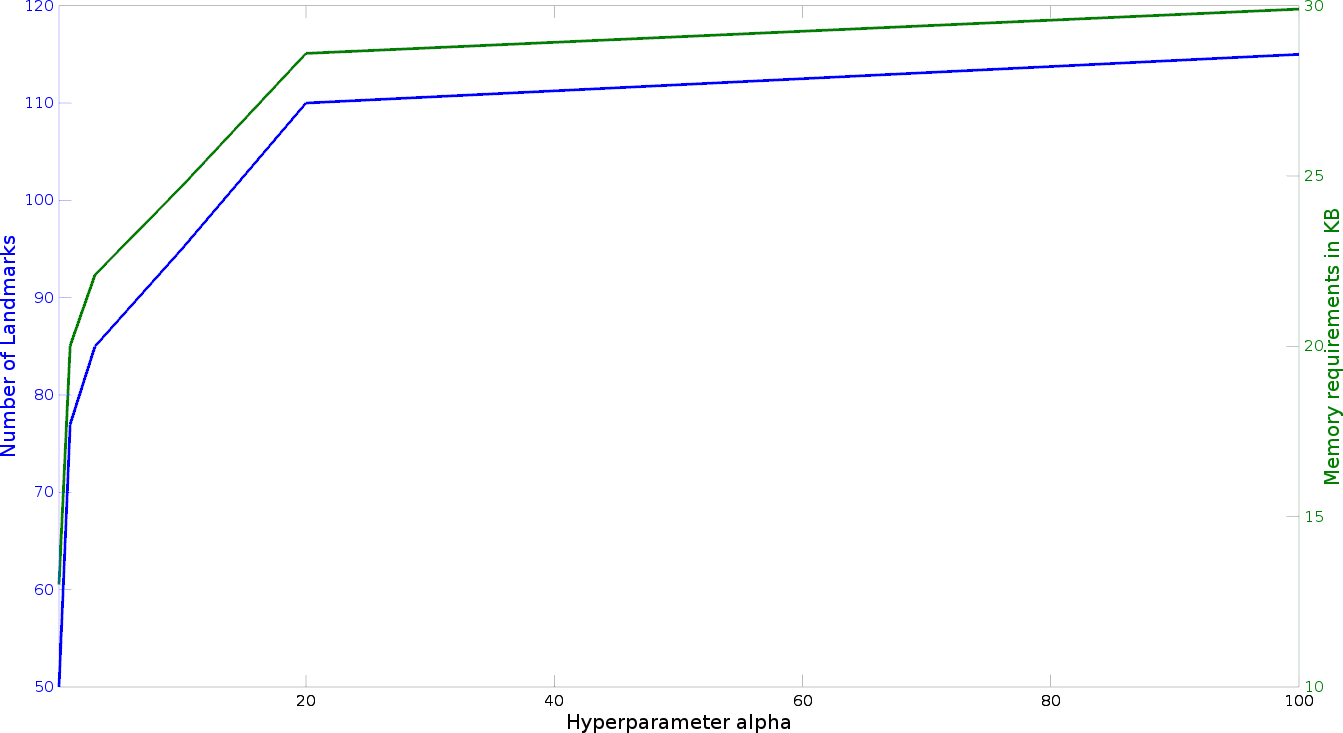
\includegraphics[width=.8\textwidth]{memoryRequirements2}
    \caption{Memory Requirements as a function of strength parameter $\alpha$.}
  \label{memReq}
\end{figure}

\begin{figure}[ht!]
  \centering
    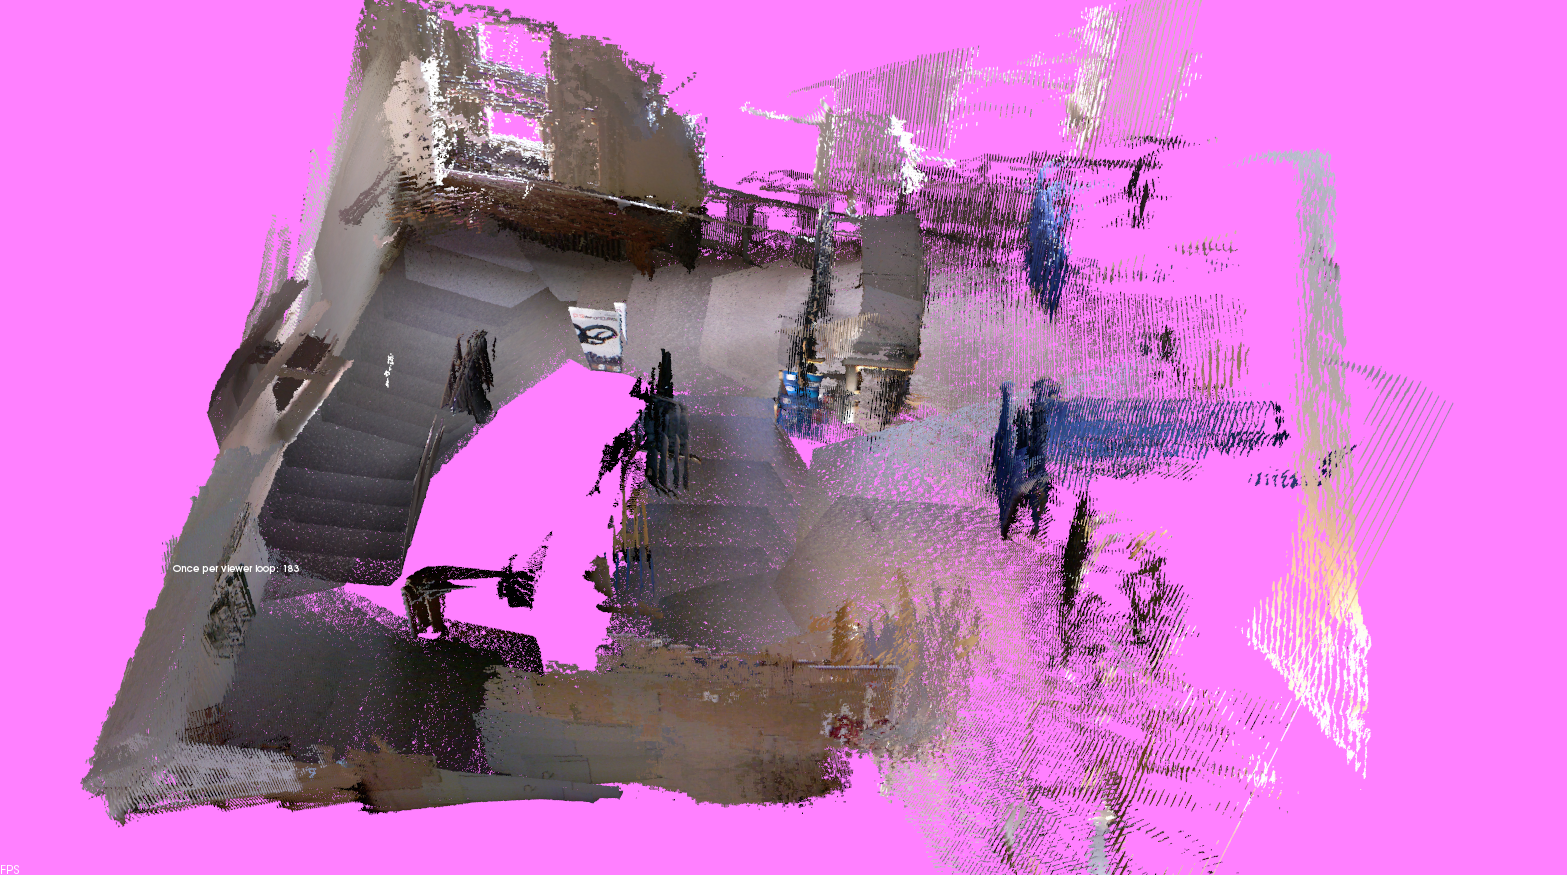
\includegraphics[width=.8\textwidth]{rtabmap}
    \caption{Result of a session using RTAB-map module. The resulting map captures the structure of the room and the maps for the room shown in the picture average 84MB in size.}
  \label{rtabmap}
\end{figure}

As can be seen, the number of landmarks follows the logarithmic trend of the distribution in relation to $\alpha$.
Increasing the $\alpha$ value more will not make the algorithm follow the logarithmic trend indefinitely. 
That is due to the fact that as the $\alpha$ increases, the constant decision layer has an upper bound to the number of landmarks it can support. 
This means that the algorithm will keep adding landmarks until the environment saturates and no new landmarks can be added.
It must also be noted that as the $\alpha$ parameter is set to higher values, the sampler outputs more clusters making it a more accurate environment descriptor.
On the other hand, having a high hyperparameter $\alpha$ increases the computation time of the sampler, making it non feasible to use in real time mapping scenarios.
Values of $\alpha$ between 1 and 10 provide a robust but also fast enough sampler that can be used in online mapping scenarios.


\newpage
\section{Discussion}
\label{sec:discussion}

The discussion section investigates modelling choices like the data distribution, details regarding specific parts of the pipeline, as well as implications that are part of the theoritical background the pipeline is build on. Finally some limits of the pipeline in relation to the parameter values it uses are investigated.

 
\subsection{Data distribution}

One of the fundamental properties of the model is the data distribution it infers. 
The data distribution that was introduced and analyzed in \ref{data:dist} and is an extension to the distribution proposed in \cite{dependentDiri} for 2D video data.
The object distribution was chosen to be simple but also expressive enough to be able to handle the information the environment contains efficiently.
If the problem definition was formulated differently, alternative features could be used and, consequently, a different environment distribution could be used instead.
More complex environment distributions can lead to objects that capture the information of the environment contains with a higher amount of precision. 
The memory requirements for every extra component will then increase with respect to the number of parameters the conjugate distribution of the component requires. 
 
\subsection{Downsampling and Filtering}

The downsampling and filtering operations are important as they affect the speed of sampling and the quality of clusters the infered on every iteration. 
During those operations the cloud is transformed from raw kinect readings to the data the sampler expects.
Downsampling is used to reduce the size of the cloud and increase the speed of the method since the complexity of the pipeline is directly related to cloud size as it was shown in section \ref{subsec:complexity}. Filtering operations calculate the features for every point of the downsampled cloud.
Having the downsampling operations run on a low threshold will lead to a large cloud after the downsampling takes place. 
Passing a large cloud in the sampler will result in a more precise environment representation, but also a slower clustering process.
On the other hand, having downsampling operations run with a very high threshold will lead to a very small cloud that has a very small amount of information the inital cloud carried. This will lead to clustering results that do not contain significant information regarding the initial cloud.

Fig.\ref{pip:downsample} displays the results of having the pipeline run with a high(a) and a low(b) threshold on the milk cartridge dataset that was introduced in Fig.\ref{pcl:clust}(a).
The first figure displays a cloud that has a small amount of points removed during the downsampling operations. The sampler will then receive a cloud with a lot of the initial information still contained in its structure.
The second figure displays a cloud that has keept a very small portion of the points the initial cloud carried.


\begin{figure}[!ht]
\begin{tabular}{cc}
    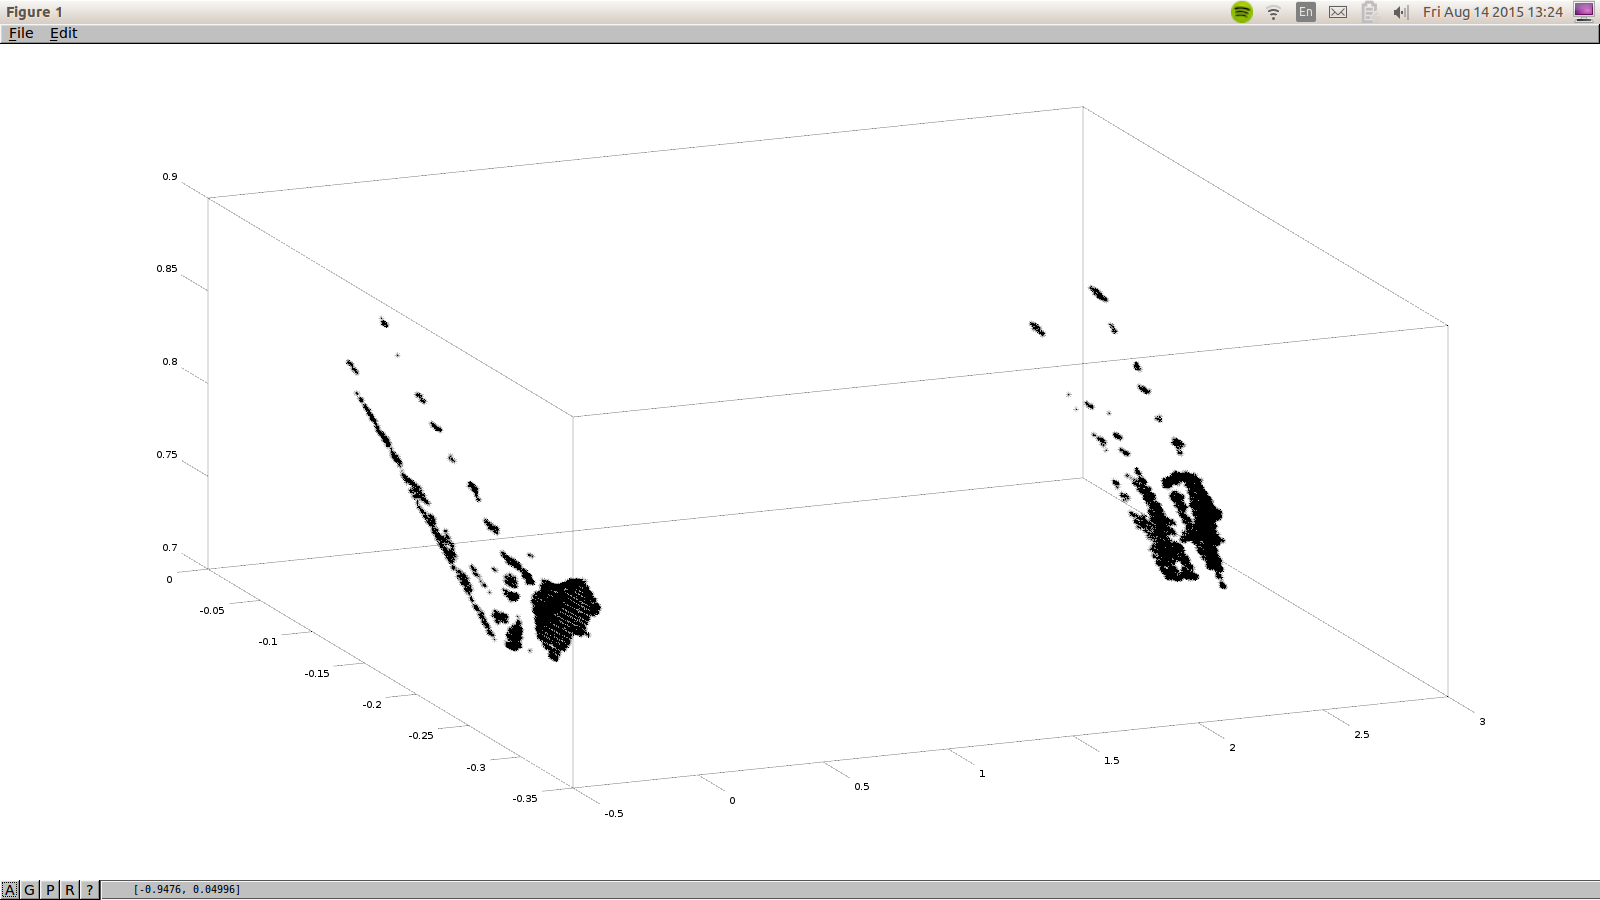
\includegraphics[width=.4\textwidth]{smalldownsamplinglimit} &  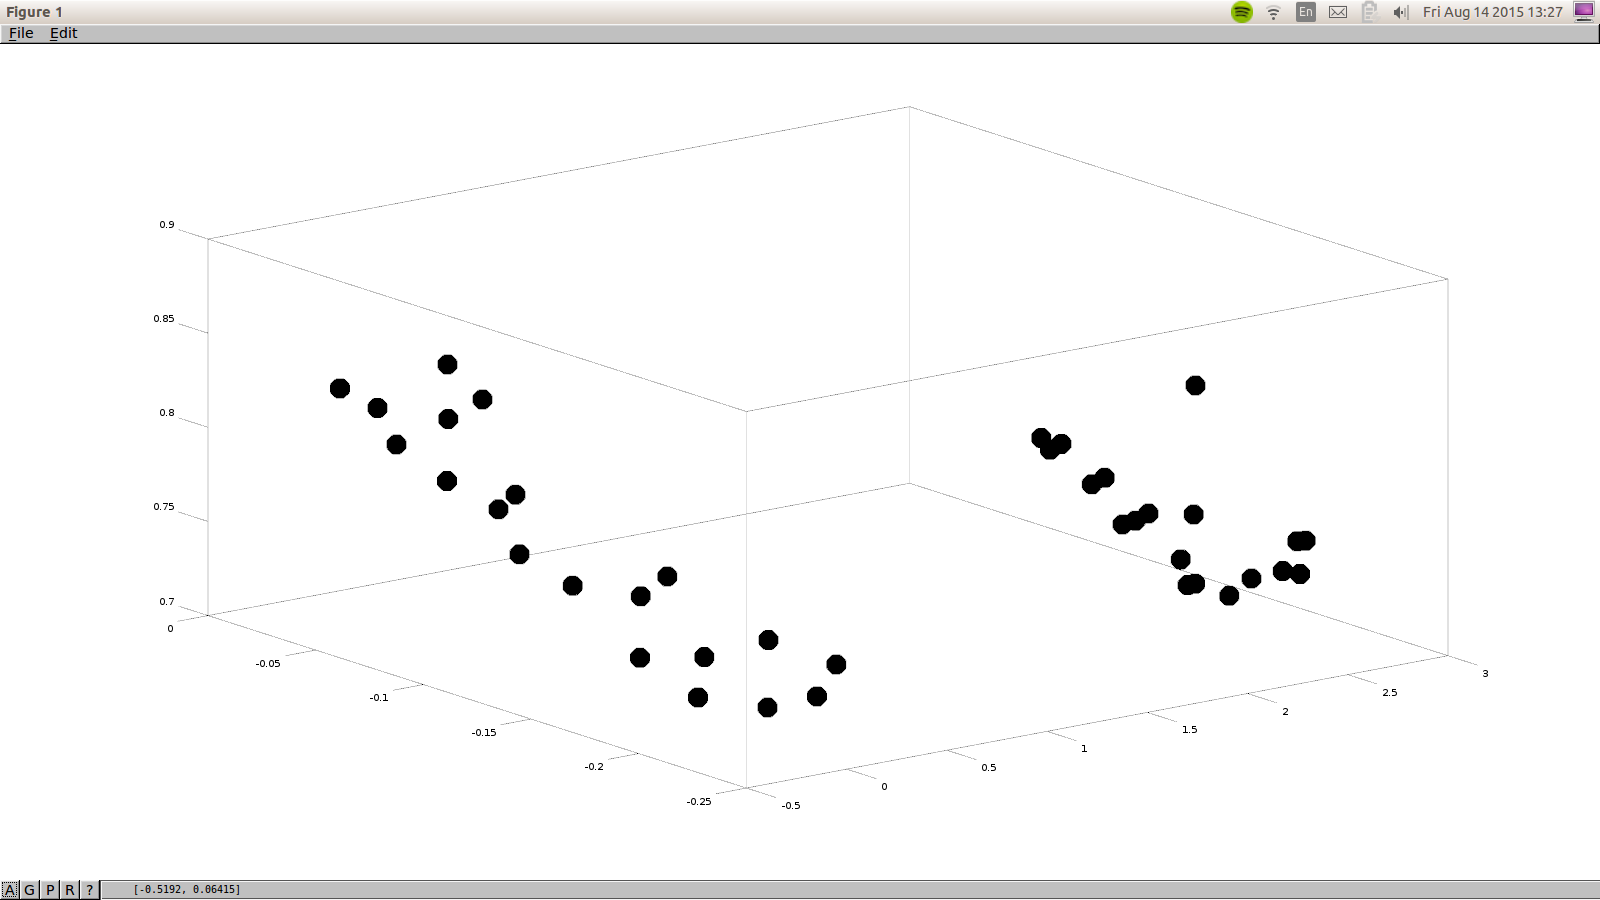
\includegraphics[width=.4\textwidth]{largedownsamplinglimit} \\
    (a) Small threshold in the downsampling  & (b) A high threshold in the downsampling  \\
        leads to  a high amoung of points    &     leads to a small amount of poits \\
        propagated to the sampler            &     propagated to the sampler  \\[6pt]
\end{tabular}
\caption{The behaviour of the dowsampling module with respect to the threshold of the operations.}
  \label{pip:downsample}
\end{figure}
  
\subsection{Unsupervised learning}


It is important to note the implications of having a pipeline that is based on a Dependent Dirichlet Process i.e. an unsupervised learning algorithm. Due to the unsupervised nature of the method, the elements of the cloud will be clustered as the algorithm sees (statistically)fit. This means that there will be clusters in the cloud that will be small in size and will contain just parts of an object and, conversely, clusters that are large contain more than a single object. The environment is therefore clustered in chunks that need not be semantically sound. One such example is shown in Fig.\ref{pip:beh} where multiple milk cartridges are either clustered as single entities or part of larger clusters.

This is an expected behaviour given the unsupervised nature of the method and it does not hinder the results of the pipeline. In projects where the focus is directed towards individuating parts of the environment with higher degree of precision, more complex object signatures can be used to force the sampler in only grouping only parts of the environment that share a high amount of homogeneity among their features. If classification of objects nececary a decision layer could be added on top of the clustering and objects could be classified on the distribution level. Unsupervised approaches make the method general and able to handle a high amount of different environments. 


\begin{figure}[!ht]
\begin{tabular}{cc}
    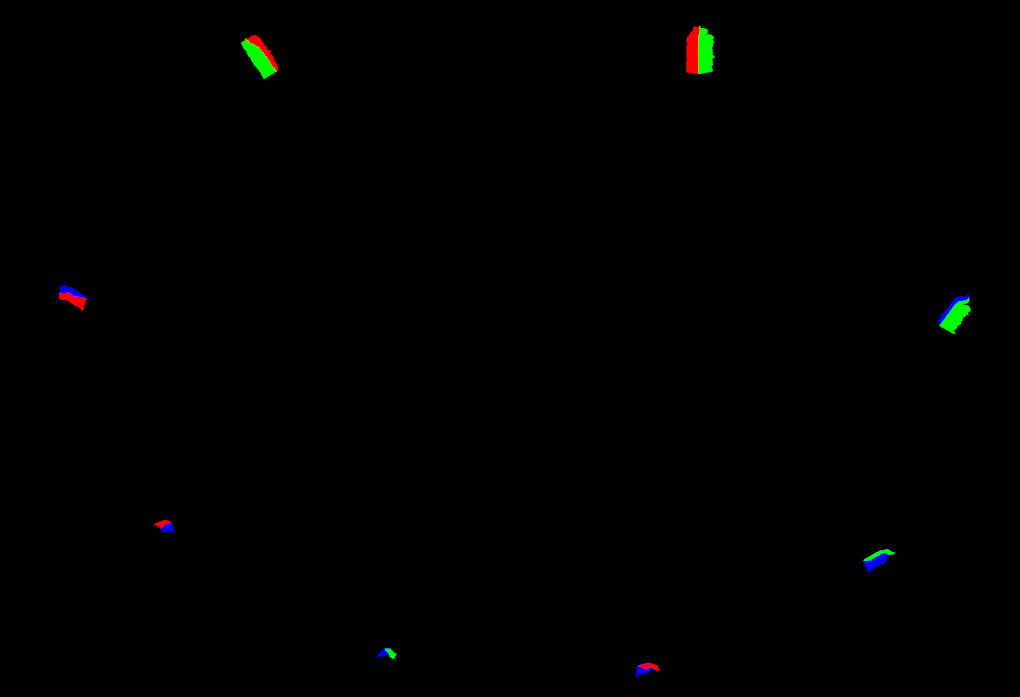
\includegraphics[width=.5\textwidth]{8boxesData} &  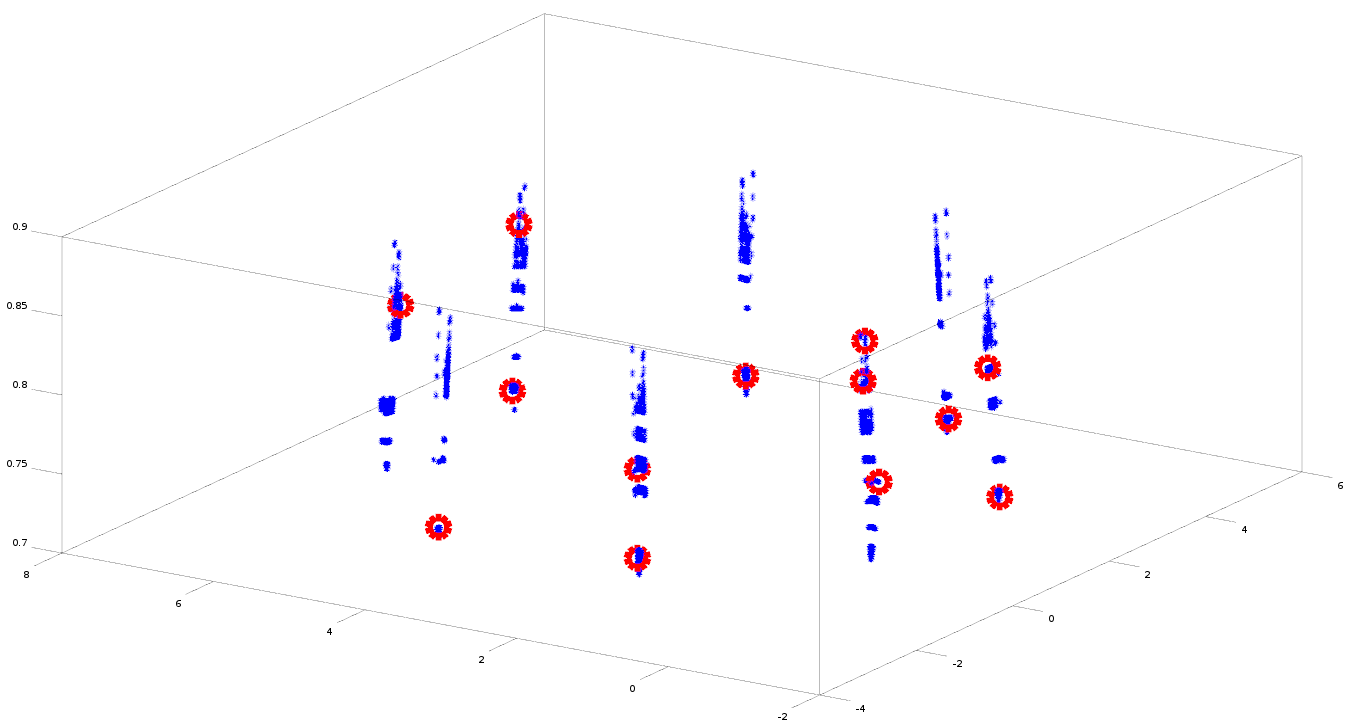
\includegraphics[width=.5\textwidth]{8boxes} \\
  (a) Initial data  & (b) Clusters infered \\[6pt]
\end{tabular}
\caption{Unsupervised entity extraction.}
  \label{pip:beh}
\end{figure}


\subsection{Clustering layer}

An important property regarding the behaviour of the pipeline exists with respect to the Dirichlet hyperparameter $\alpha$. During the clustering, choosing a correct value for the hyperparameter $\alpha$ is important. When the sampler is run with a very low $\alpha$, the whole cloud will be assigned to a small amount of clusters, or, in the extreme case, a single cluster. Having every point in the cloud assigned to the same cluster leads to a a significant amount of information loss as no region specific information is passed to the clusters output. Fig.[\ref{pip:limits}] shows the behaviour of the sampler for $\alpha$ values lower than 1. The clusters are color coded in the downsampled cloud, and it can be seen that only one cluster is output by the sampler.

On the other hand, having a very large $\alpha$ can lead to a very large amount of clusters being output by the sampler on every iteration of the method. That can lead to a non converging pipeline since every time a new landmark that does not fit the landmark database is output. This leads to many small clusters with each one containing a small number of points. Furthermore, setting a high $\alpha$ value leads to a slower sampling process since the complexity of the sampler is $O(TKLSN)$ where $K$ is defined as the number of clusters. Fig.[\ref{pcl:kl}] displays the behavior of the sampler for very large values $\alpha$. The landmarks extracted from a single cloud are shown as spheres; it can be seen that the cloud is not visible and the majority of the points is considered as standalone landmarks.

Both such behaviours are expected and can be explained from the theory on Dirichlet processes\cite{dependent}. Generally, in every application the value choice of hyperparameter $\alpha$ will affect the precision of the sampler. If the task at hand requires a high amount of precision, the sampler can be run with a high hyperparameter $\alpha$. That way every point will become a cluster minimizing information loss with respect to the cloud. Having a low $\alpha$ forces the sampler to group a high amount of points in the dataset together. That leads to a high amount of information loss and is not usefull in most scenarios. If the domain in which the sampler is run requires fast decision making, the sampler could be run with a smaller value of $\alpha$. That way it would ouput a smaller amount of clusters and would consequently be faster. Since the information loss is larger compared to high-alpha runs, tweaking the value of $\alpha$ is a task usually left on the user and is related to  what the corresponding problem at hand is. Given that one basic motivation of this thesis was a method that could be used in online SLAM problems, small initial values of $\alpha$ in the range of 1-10 were used. That way the sampler was fast while the information loss was manageable.

\begin{figure}
\begin{tabular}{cc}
    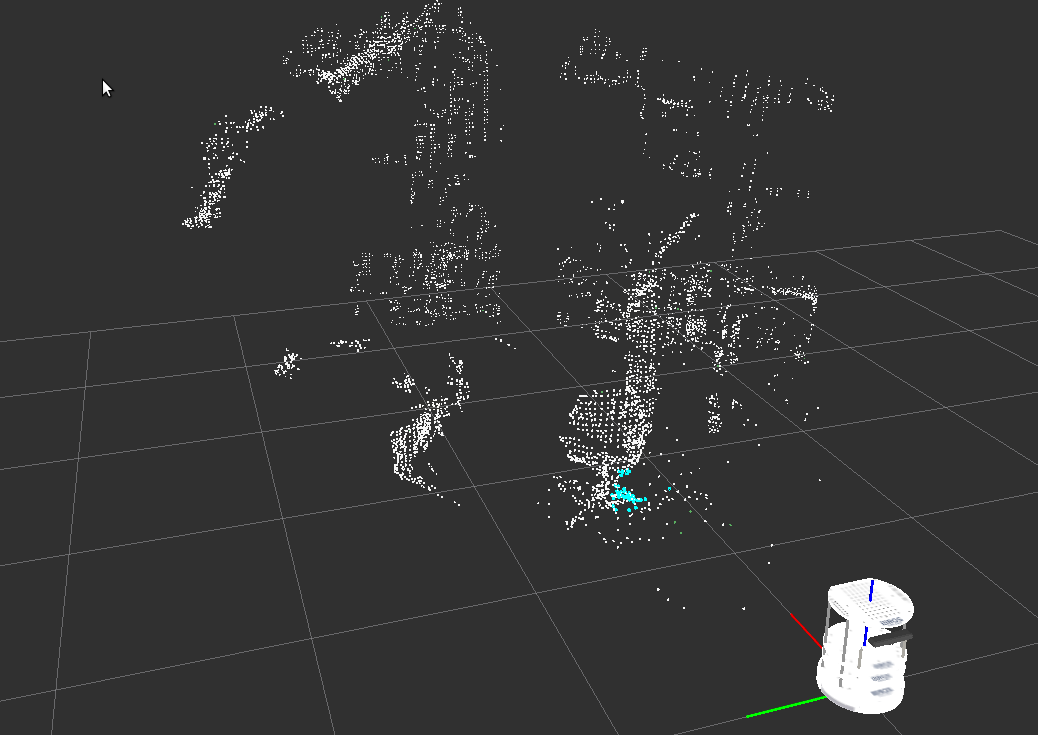
\includegraphics[width=.5\textwidth]{singlecluster} &  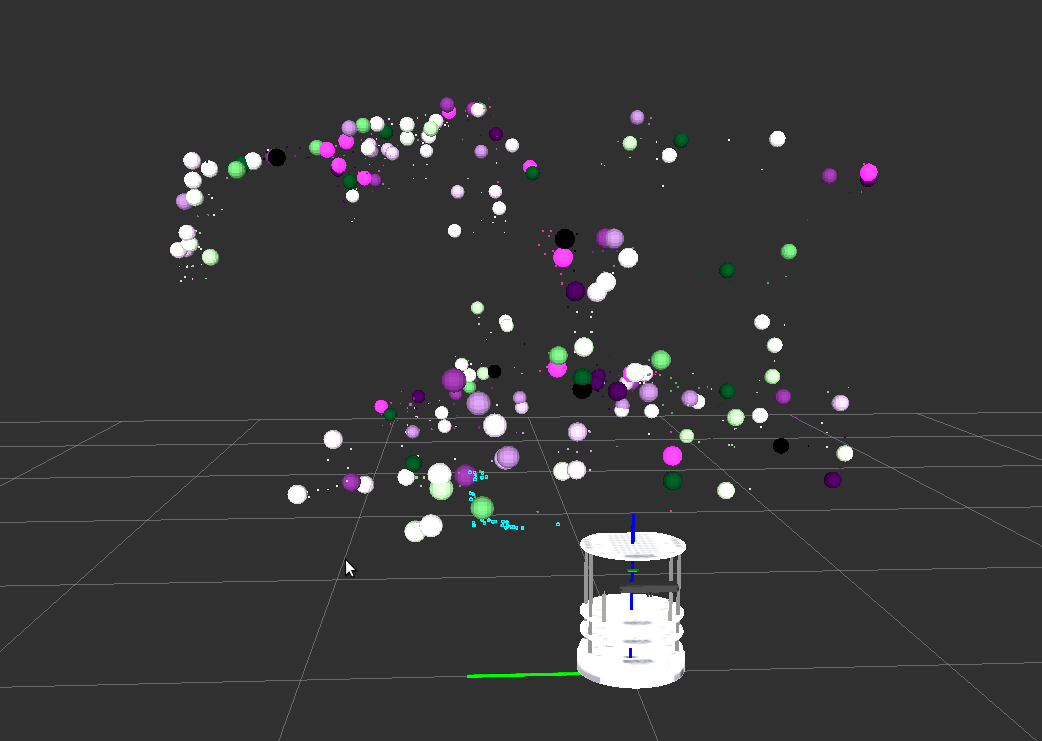
\includegraphics[width=.5\textwidth]{onlyclusters2} \\
  (a) Low $\alpha$ translates to a single cluster  & (b) High $\alpha$ translates to a non converging cloud \\[6pt]
\end{tabular}
\caption{Cases where using very low/high values on the hyperparameter $\alpha$ lead to a pipeline that either groups the whole cloud being to a single landmark or to a pipeline that constantly creates new landmarks.}
  \label{pip:limits}
\end{figure}

\subsection{Decision layer}


The decision layer subsection will investigate the limits of the method that are introduced by the decision layer of the pipeline.
The restrictions introduced by the decision layer are relatively straightforward. Taking very small distances in the distance threshold operation can lead to pipeline that continuously adds new landmarks to the database. 

Such restrictions can be introduced to every part of the distances between distributions calculated in section \ref{distancesofclusters}. Taking a strict limit regarding the Gaussian counterparts will lead to a decision layer that only matches neighbor clusters. In the same way, taking a strict limit with respect to the categorical counterparts will lead to a decision making process that only matches elements with similar color signatures. Finally, taking a strict exponential limit will lead to a decision layer that only accepts clusters with very similar angle signatures.
The exponential part is the most suspectible to noise and Fig.\ref{pip:expo} illustrates this specific behavior.

It can be seen that limiting the landmark matching operation to very small exponential distances between clusters, can lead to a cloud where a single object can be decomposed to many entities. Spheres represent landmarks and it can be seen that the chair is being assigned to many landmarks using the pipeline with this setup. That means that very strict limits lead to a non converging pipeline with respect to the landmarks it outputs. The same also holds for the rest of the distances with the Gaussian and categorical parts being less susceptible to noise. 

Furthermore, since the number of landmarks is also a function of noise, areas of the cloud that are near the maximum range of the sensor can lead to different landmarks added frequently. These issues can be tackled by having a less strict limit in the operation that defines what is considered a landmark the sampler has encountered before or not.

\begin{figure}[!ht]
        \centering
	    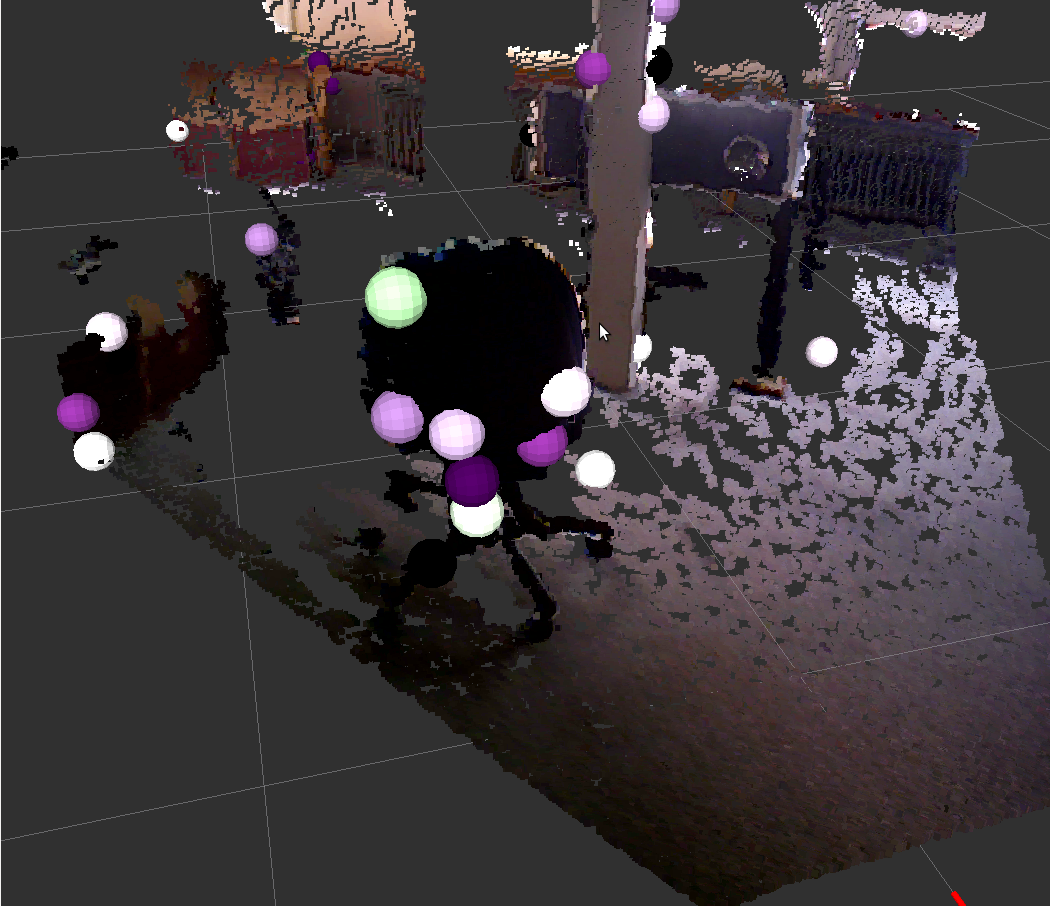
\includegraphics[width=.5\textwidth]{monsterchair} \\
	  (a) Very strict decision limits lead to multiple \\
	   entities on a single \\[6pt]
	  \label{pip:expo}
\end{figure}

\subsection{Scalability}

The repesentation introduced is scalable with respect to its memory needs and the landmark matching operations as the number of landmarks in the environment increases.
The small amount of memory a single landmark singature requires(260Bytes) makes the method capable of handling a large amount of landmarks. Fig.\ref{pip:reqs} displays the memory requirements in relation to the number of landmarks in the environment. It can be seen that even for a very large amount of landmarks(>1000) the memory requirements are low(<10MB).

Furthermore, when a high amount of  landmarks is introduced in the system, there exists a number of techniques that can be used to reduced the time required for the landmark matching operations.
For example, since landmarks are stored in a database, only landmarks occupying a specific part of the map can be retrieved;
that way the landmark matching operations will be constant with respect to the number of landmarks the decision layer allows in a specific part of the map. 

\begin{figure}[!ht]
  \centering
  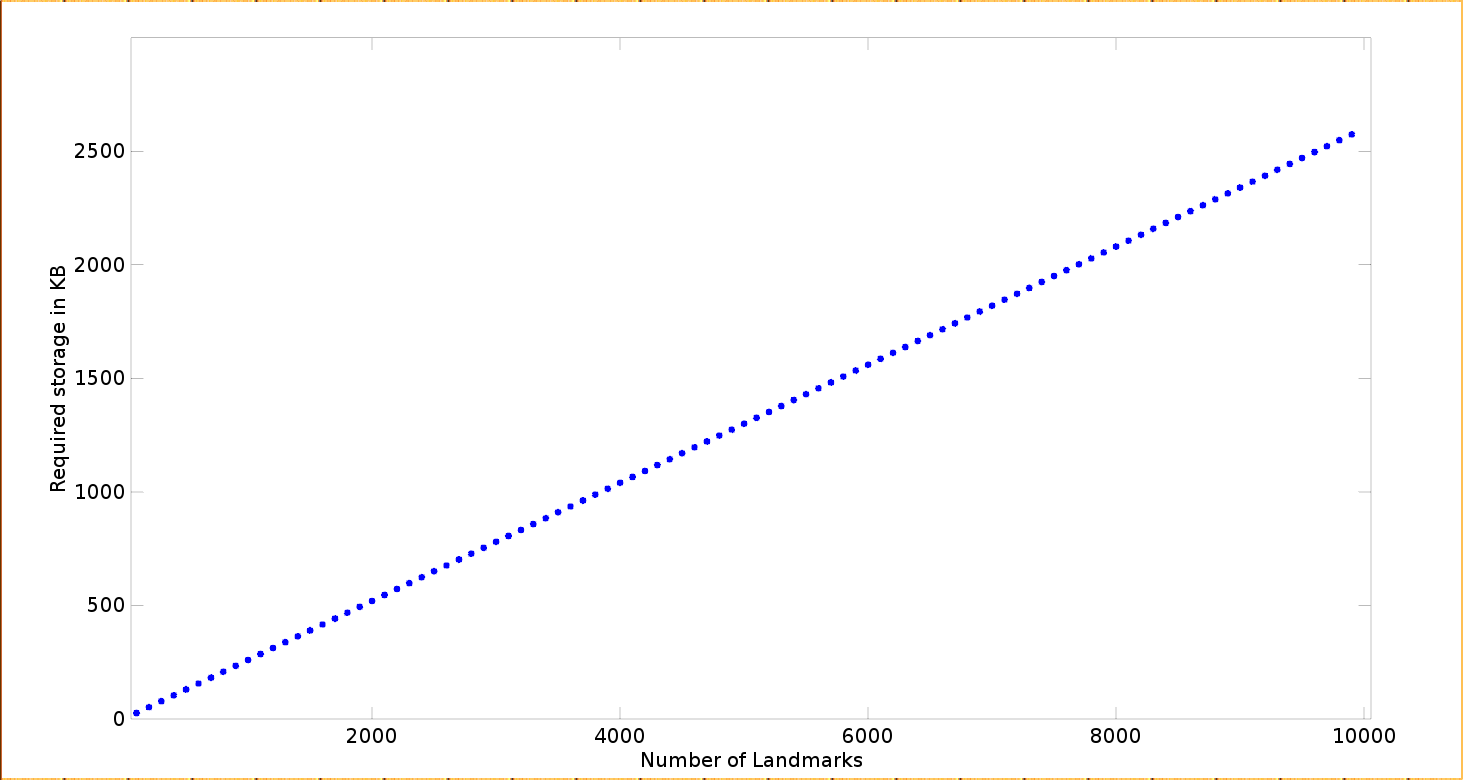
\includegraphics[width=.8\textwidth]{MemoryRequirements} \\
  \caption{Memory requirements with respect to the number of landmarks in the environment. 10000 landmarks have memory needs of 2.6MB making the method very memory efficient.}
  \label{pip:reqs}
\end{figure}


\newpage
\section{Conclusion and future work}
\label{sec:conclusion}

In this thesis a novel cloud representation by using Bayesian methodologies was introduced.
An application of the representation was introduced through a pipeline that uses this representation as a sensor model in landmark based slam. 

Representation signatures were presented first on simple datasets and were analyzed towards their results. 
The decision layer section displayed the expressive capabilities of the signature and how it distinguishes between different parts of the environment.
In order to show the extend of the expressiveness of the method, the pipeline was then used as the sensor model of a landmark based EKF-SLAM algorithm.
The pipeline was then tested towards its speed on two different machines.
Finally, the memory needs of amapping using this method were investigated and it was shown that the number of landmarks follows the logarithmic trend of the underlying Dirichlet distribution until the environment saturates on landmarks.

 The discussion section investigated the implications of using a pipeline that is build on top of an unsupervised learning method. 
 The motivation behind using such data signature was analyzed and how more demanding problems can lead to more complex environment signatures that better represent environment signatures.
 Furthermore the importance of hyperparameter $\alpha$ was analyzed as well as how should the $\alpha$ value be chosen with respect to the problem at hand. Having a correct $\alpha$ value is important since it can lead the pipeline to produce sub-optimal results. 
 With respect to the downsampling process, the discussion section analyzed how the tweaking of the downsampling parameters helps the user choose between speed and precision in the pipeline.
 Finally, the scalability of the pipeline was presented along with examples of how the landmark matching operations could handle an increasing number of landmarks in an environment.

There are a number of directions in which the pipeline can be improved.
Choosing more complex environment signatures could increase the expresional strength of the sampler making it more robust and capable of to representing with higher precision more complex structures.
Furthermore, since the sampler clusters parts of environment, it would be interesting to see how a hierarchical approach would affect the result of the clustering.
Hierarchical dependent Dirichlet processes would be interesting extensions since such tools would both have the ability to capture structures in a hierarchal way not just as chunks of the environment as well as be able to handle the dynamic component that lifelong mapping problems introduce. 
Furthermore, having a more complex decision layer would also increase the robustness of the method making it able to handle more complex environment structures. 
Finally, all those additions could help tackle lifelong mapping problem as a whole in a fully Bayesian manner.


%------------------------------------------------


\begin{thebibliography}{9}

\bibitem{probRobs}
\newblock Thrun, S. (2002). Probabilistic robotics. Communications of the ACM, 45(3), 52-57.


\bibitem{ekf}
\newblock Bailey, T., Nieto, J., Guivant, J., Stevens, M., \& Nebot, E. (2006, October). Consistency of the EKF-SLAM algorithm. In Intelligent Robots and Systems, 2006 IEEE/RSJ International Conference on (pp. 3562-3568). IEEE.

\bibitem{graph}
\newblock Thrun, S., \& Montemerlo, M. (2006). The graph SLAM algorithm with applications to large-scale mapping of urban structures. The International Journal of Robotics Research, 25(5-6), 403-429.

\bibitem{Figueredo:2009dg}
Figueredo, A.J. and Wolf, P. S.A. (2009).
\newblock Assortative pairing and life history strategy - a cross-cultural
  study.
\newblock {\em Human Nature}, 20:317--330.

\bibitem{liflonglearning}
\newblock Thrun, S., \& Mitchell, T. M. (1995). Lifelong robot learning. The Biology and Technology of Intelligent Autonomous Agents, 165-196.

\bibitem{lifelongmaps}
\newblock Konolige, K., \& Bowman, J. (2009, October). Towards lifelong visual maps. In Intelligent Robots and Systems, 2009. IROS 2009. IEEE/RSJ International Conference on (pp. 1156-1163). IEEE.

\bibitem{aishalong}
\newblock Walcott, A. (2011). Long-term robot mapping in dynamic environments (Doctoral dissertation, Massachusetts Institute of Technology).

\bibitem{bayesianNon}
\newblock Hjort, N. L., Holmes, C., Müller, P., \& Walker, S. G. (Eds.). (2010). Bayesian nonparametrics (Vol. 28). Cambridge University Press.

\bibitem{dependent}
\newblock {MacEachern, S. N. (2000) Dependent dirichlet processes. Unpublished manuscript, Department of Statistics, The Ohio State University.}

\bibitem{brml}
\newblock{Barber, D. (2012) Bayesian reasoning and machine learning.}

\bibitem{dependentDiri}
\newblock{Neiswanger, W., Wood, F., \& Xing, E.The dependent dirichlet process mixture of objects for detection-free tracking and object modeling. In Proceedings of the Seventeenth International Conference on Artificial Intelligence and Statistics (pp. 660-668) (2014, August) }

\bibitem{pcl}
\newblock{Rusu, R. B., \& Cousins, S. (2011, May). 3d is here: Point cloud library (pcl). In Robotics and Automation (ICRA), 2011 IEEE International Conference on (pp. 1-4). IEEE.}

\bibitem{rtabmap}
\newblock Labbé, M., \& Michaud, F. (2011, September). Memory management for real-time appearance-based loop closure detection. In Intelligent Robots and Systems (IROS), 2011 IEEE/RSJ International Conference on (pp. 1271-1276). IEEE.


\bibitem{SLAM++}
\newblock Salas-Moreno, R. F., Newcombe, R. A., Strasdat, H., Kelly, P. H., \& Davison, A. J. (2013, June). Slam++: Simultaneous localisation and mapping at the level of objects. In Computer Vision and Pattern Recognition (CVPR), 2013 IEEE Conference on (pp. 1352-1359). IEEE.

\bibitem{objSLAM}
\newblock Selvatici, A. H., \& Costa, A. H. (2008). Object-based visual SLAM: How object identity informs geometry.

\bibitem{castleetal}
\newblock Castle, R. O., Gawley, D. J., Klein, G., \& Murray, D. W. (2007, April). Towards simultaneous recognition, localization and mapping for hand-held and wearable cameras. In Robotics and Automation, 2007 IEEE International Conference on (pp. 4102-4107). IEEE.


\bibitem{objectpointSLAM}
\newblock Choudhary, S., Trevor, A. J., Christensen, H. I., \& Dellaert, F. (2014, September). SLAM with object discovery, modeling and mapping. In Intelligent Robots and Systems (IROS 2014), 2014 IEEE/RSJ International Conference on (pp. 1018-1025). IEEE.

\bibitem{objectpoint}
\newblock Jensfelt, P., Ekvall, S., Kragic, D., \& Aarno, D. (2006, September). Augmenting SLAM with object detection in a service robot framework. In Robot and Human Interactive Communication, 2006. ROMAN 2006. The 15th IEEE International Symposium on (pp. 741-746). IEEE.

\bibitem{monoSLAM}
\newblock Davison, A. J., Reid, I. D., Molton, N. D., \& Stasse, O. (2007). MonoSLAM: Real-time single camera SLAM. Pattern Analysis and Machine Intelligence, IEEE Transactions on, 29(6), 1052-1067.

\bibitem{objectDisc}
\newblock Koo, S., Lee, D., \& Kwon, D. S. (2014, September). Unsupervised object individuation from RGB-D image sequences. In Intelligent Robots and Systems (IROS 2014), 2014 IEEE/RSJ International Conference on (pp. 4450-4457). IEEE.


\bibitem{distMes}
\newblock{Cichocki, A., \& Amari, S. I.Families of alpha-beta-and gamma-divergences: Flexible and robust measures of similarities. Entropy, 12(6), 1532-1568.}

\bibitem{fpfh}
\newblock{Fast point feature histogram.Rusu, R. B., Blodow, N., \& Beetz, M. (2009, May). Fast point feature histograms (FPFH) for 3D registration. In Robotics and Automation, 2009. ICRA'09. IEEE International Conference on (pp. 3212-3217). IEEE.}

\bibitem{segOverview}
\newblock {Rabbani, T., van den Heuvel, F., \& Vosselmann, G. (2006). Segmentation of pointclouds using smoothness constraint. International Archives of Photogrammetry, Remote Sensing and Spatial Information Sciences, 36(5), 248-253.}

\bibitem{gpu}
\newblock{Caron, F., Davy, M., \& Doucet, A. (2012) Generalized Polya urn for time-varying Dirichlet process mixtures. arXiv preprint arXiv:1206.5254.}


\bibitem{kinect}
\newblock{Zhang, Z. (2012) Microsoft kinect sensor and its effect. MultiMedia, IEEE, 19(2), 4-10.}

\bibitem{nonParam}
\newblock{Wainwright, M. J., \& Jordan, M. I. (2008). Graphical models, exponential families, and variational inference. Foundations and Trends in Machine Learning, 1(1-2), 1-305.}
``
\bibitem{omnimaper}
\newblock{A.Trevor,  J.Rogers, and  H.Christensen.  Omnimapper:  A  modular multimodal  mapping  framework.   In IEEE  International  Conference on Robotics and Automation (ICRA), 2014}

\bibitem{imft}
\newblock Koo, S., Lee, D., \& Kwon, D. S. (2013, November). Multiple object tracking using an rgb-d camera by hierarchical spatiotemporal data association. In Intelligent Robots and Systems (IROS), 2013 IEEE/RSJ International Conference on (pp. 1113-1118). IEEE.

\bibitem{pointSeg}
\newblock Trevor, A. J., Gedikli, S., Rusu, R. B., \& Christensen, H. I. (2013). Efficient organized pointcloud segmentation with connected components. Semantic Perception Mapping and Exploration (SPME).

\bibitem{planarSeg}
\newblock Unnikrishnan, R., \& Hebert, M. (2003, October). Robust extraction of multiple structures from non-uniformly sampled data. In Intelligent Robots and Systems, 2003.(IROS 2003). Proceedings. 2003 IEEE/RSJ International Conference on (Vol. 2, pp. 1322-1329). IEEE. 

\bibitem{planarSeg2}
\newblock Rabbani, T., van den Heuvel, F., \& Vosselmann, G. (2006). Segmentation of pointclouds using smoothness constraint. International Archives of Photogrammetry, Remote Sensing and Spatial Information Sciences, 36(5), 248-253.

\bibitem{smartSeg}
\newblock Triebel, R., Shin, J., \& Siegwart, R. (2010, June). Segmentation and unsupervised part-based discovery of repetitive objects. In Robotics: Science and Systems (Vol. 2).

\bibitem{smcddp}
\newblock Neiswanger, W., Wood, F., \& Xing, E. (2014, August). The dependent dirichlet process mixture of objects for detection-free tracking and object modeling. In Proceedings of the Seventeenth International Conference on Artificial Intelligence and Statistics (pp. 660-668).

\bibitem{corresp:first}
\newblock Cree, M. J., Jefferies, M. E., \& Baker, J. T. Using 3D Visual Landmarks to Solve the Correspondence Problem in Simultaneous Localisation and Mapping.

\bibitem{corres:sec}
\newblock Lowe, D. G. (2004). Distinctive image features from scale-invariant keypoints. International journal of computer vision, 60(2), 91-110.

\bibitem{corres:three}
\newblock Lamon, P., Tapus, A., Glauser, E., Tomatis, N., \& Siegwart, R. (2003, October). Environmental modeling with fingerprint sequences for topological global localization. In Intelligent Robots and Systems, 2003.(IROS 2003). Proceedings. 2003 IEEE/RSJ International Conference on (Vol. 4, pp. 3781-3786). IEEE.


\bibitem{corres:four}
\newblock Sehgal, A., Cernea, D., \& Makaveeva, M. (2010). Real-time scale invariant 3D range pointcloud registration. In Image Analysis and Recognition (pp. 220-229). Springer Berlin Heidelberg.

\bibitem{bayes:neal}
\newblock Neal, R. M. (2000). Markov chain sampling methods for Dirichlet process mixture models. Journal of computational and graphical statistics, 9(2), 249-265.

\bibitem{bayes:jordan}
\newblock Blei, D. M., \& Jordan, M. I. (2006). Variational inference for Dirichlet process mixtures. Bayesian analysis, 1(1), 121-143.

\bibitem{SLAM}
\newblock{Montemerlo, M., Thrun, S., Koller, D., \& Wegbreit, B. (2002). FastSLAM: A factored solution to the simultaneous localization and mapping problem. AAAI/IAAI, 593-598.}

\bibitem{bayes:hier}
\newblock Teh, Y. W., Jordan, M. I., Beal, M. J., \& Blei, D. M. (2006). Hierarchical dirichlet processes. Journal of the american statistical association, 101(476).

\bibitem{bayes:smc}
\newblock Doucet, A., De Freitas, N., \& Gordon, N. (2001). An introduction to sequential Monte Carlo methods (pp. 3-14). Springer New York.

\bibitem{LDA}
\newblock{Blei, D. M., Ng, A. Y., \& Jordan, M. I. (2003). Latent dirichlet allocation. the Journal of machine Learning research, 3, 993-1022.}

\bibitem{theory:ddp}
\newblock MacEachern, S. N. (2000). -
\bibitem{speakerDiar}
\newblock{Fox, E. B., Sudderth, E. B., Jordan, M. I., \& Willsky, A. S. (2011). A sticky HDP-HMM with application to speaker diarization. The Annals of Applied Statistics, 5(2A), 1020-1056.}


\bibitem{antoniak}
\newblock{Charles E Antoniak,Mixtures of dirichlet processes with applications to bayesian nonparametric problems, The annals of statistics (1974), 1152–1174}

\bibitem{caron}
\newblock{F. Caron, M. Davy, and A. Doucet, Generalized Polya urn for time-varying Dirichlet process mixtures, 23rd Conference on
Uncertainty in Artificial Intelligence (UAI’2007), Vancouver,
Canada, July 2007, 2007}

\bibitem{compendium}
\newblock{Fink, D. (1997). A compendium of conjugate priors.}

\bibitem{smc:theory}
\newblock{Ülker, Y., Günsel, B., \& Cemgil, A. T. (2010). Sequential Monte Carlo samplers for Dirichlet process mixtures. In International Conference on Artificial Intelligence and Statistics (pp. 876-883).}

\bibitem{doucet}
\newblock{Del Moral, P., Doucet, A., \& Jasra, A. (2006). Sequential monte carlo samplers. Journal of the Royal Statistical Society: Series B (Statistical Methodology), 68(3), 411-436.}

\bibitem{RANSAC}
\newblock{Meer, P., Mintz, D., Rosenfeld, A., \& Kim, D. Y. (1991). Robust regression methods for computer vision: A review. International journal of computer vision, 6(1), 59-70.}

\bibitem{conjugate}
\newblock Raiffa, H. (1974). Applied statistical decision theory.

\bibitem{sqlite}
\newblock{https://www.sqlite.org/datatype3.html}

\bibitem{polya}
\newblock{Johnson, N. L., \& Kotz, S. (1977). Urn models and their application: an approach to modern discrete probability theory (Vol. 77). New York: Wiley.}

\bibitem{infants}
\newblock{Xu, F., Carey, S., \& Welch, J. (1999). Infants' ability to use object kind information for object individuation. Cognition, 70(2), 137-166.}

\bibitem{rgbdmapping}
    \newblock{Henry, P., Krainin, M., Herbst, E., Ren, X., \& Fox, D. (2012). RGB-D mapping: Using Kinect-style depth cameras for dense 3D modeling of indoor environments. The International Journal of Robotics Research, 31(5), 647-663.}

 
\end{thebibliography}

%----------------------------------------------------------------------------------------



\end{document}
